\chapter{Progettazione}

\section{Analisi dei vincoli e scelte progettuali}

\subsection{Scelta sul tipo di dato}

Il tipo di dati che la libreria è in grado di gestire sono due:

\begin{itemize}
    \item \texttt{NumPy array}
    \item \texttt{Pandas DataFrame}
\end{itemize}

La scelta sull'utilizzo di questi due tipi di dati è stata fatta sulla base sia del fatto che sono tipi ampiamente diffusi ed utilizzati, sia per la compatibilità con la libreria \textit{Scikit-learn}.

Ogni algoritmo può quindi ricevere in ingresso dati in uno di questi due formati. Questo vincolo vale anche per tutte le altre funzionalità della libreria.


\subsection{Divisione in moduli}

La libreria è composta principalmente da cinque moduli, in modo che ogni funzionalità sia ben separata:

\begin{itemize}
    \item \texttt{preprocessing}
    \item \texttt{models}
    \item \texttt{model\_selection}
    \item \texttt{evaluation}
    \item \texttt{utils}
    \item \texttt{visualization}
\end{itemize}

I moduli di \texttt{models} e di \texttt{evaluation} sono a sua volta divisi in \texttt{implicit} e \texttt{explicit} che contengono le classi dei modelli e le funzioni di \textit{evaluation} che gestiscono i dati e i modelli con i feedback del tipo corrispondente.

\section{Preprocessing}
Il modulo contiene un serie di funzionalità che hanno lo scopo di processare i dati in modo semplice per poterli renderli adatti per i modelli. Vengono definite diverse funzioni di trasformazione che applicano una specifica trasformazione ai dati in input.

\subsection{Compatibilità con Scikit-learn del preprocessing}

Per avere compatibilità con \textit{Scikit-learn} ogni funzione di trasformazione, chiamata \textit{transformer}, deve soddisfare i seguenti requisiti:

\begin{itemize}
    \item estendere il mixin \texttt{TransformerMixin}: fornisce un'implementazione del metodo \texttt{fit\_transform} che, basata sui metodi \texttt{fit} e \texttt{transform} obbliga a definirne l'implementazione
    \begin{itemize}
        \item \texttt{fit}: impara dai dati calcolando i parametri necessari per la trasformazione. Restituisce l'istanza del \textit{transformer} stesso
        \item \texttt{transform}: applica la trasformazione ai dati usando i parametri calcolati in \texttt{fit}. Viene prodotto un nuovo \textit{DataFrame} senza modificare quello in input
        \item \texttt{fit\_transform}: esegue \texttt{fit} e poi \texttt{transform} sequenzialmente
    \end{itemize}
    \item estendere la classe \texttt{BaseEstimator}: fornisce funzionalità di base comuni a tutti gli \textit{estimator}
    \begin{itemize}
        \item implementazione automatica di \texttt{get\_params()} e \texttt{set\_params()} che rispettivamente restituiscono e impostano i parametri del \textit{transformer}
        \item supporto alla ricerca di iperparametri con \texttt{GridSearchCV} e \texttt{RandomizedSearchCV}
        \item una struttura standard per la serializzazione con \texttt{pickle} o altro
    \end{itemize}
    \item se il \textit{transformer} apprende informazioni con la chiamata al metodo \texttt{fit} allora:
    \begin{itemize}
        \item i parametri appresi devono essere settati come campi pubblici e devono terminare con il carattere "\_" (e.g. \texttt{transformer.min\_} o \\ \texttt{transformer.scale\_} per \texttt{MinMaxScaler})
        \item se durante la \texttt{fit} vengono appresi dei parametri nel metodo \texttt{transform} deve essere chiamata la funzione \texttt{check\_is\_fitted}. Questa funzione verifica la presenza di almeno un attributo il cui nome termini con il carattere ``\_'' (convenzionalmente utilizzato da \textit{Scikit-learn} per indicare che l'attributo è stato appreso durante la \texttt{fit}). In caso contrario, viene sollevata un'eccezione di tipo \texttt{NotFittedError}
    \end{itemize} 
\end{itemize}

Alcune considerazioni importanti:

\begin{itemize}
    \item in questo caso i metodi \texttt{fit}, \texttt{transform} e \texttt{fit\_transform} ricevono in ingresso solamente il tipo di dato \textit{DataFrame}, perché le trasformazioni sono specifiche per questo tipo di dato
    \item ogni \textit{transformer} è caratterizzato da specifici parametri che dipendono dal tipo di trasformazione stessa
    \item non tutti i \textit{transformers} apprendono parametri durante la \textit{fit} perché sono \textit{stateless}. In quel caso non si aggiunge il controllo con \texttt{check\_is\_fitted} all'interno della \texttt{transform}
\end{itemize}

\subsection{DataFramePreprocessFunction}

Viene definita la classe \texttt{DataFramePreprocessFunction} come estensione delle due classi sopra citate e che rappresenta una generica trasformazione.

\begin{figure}[H]
    \centering
    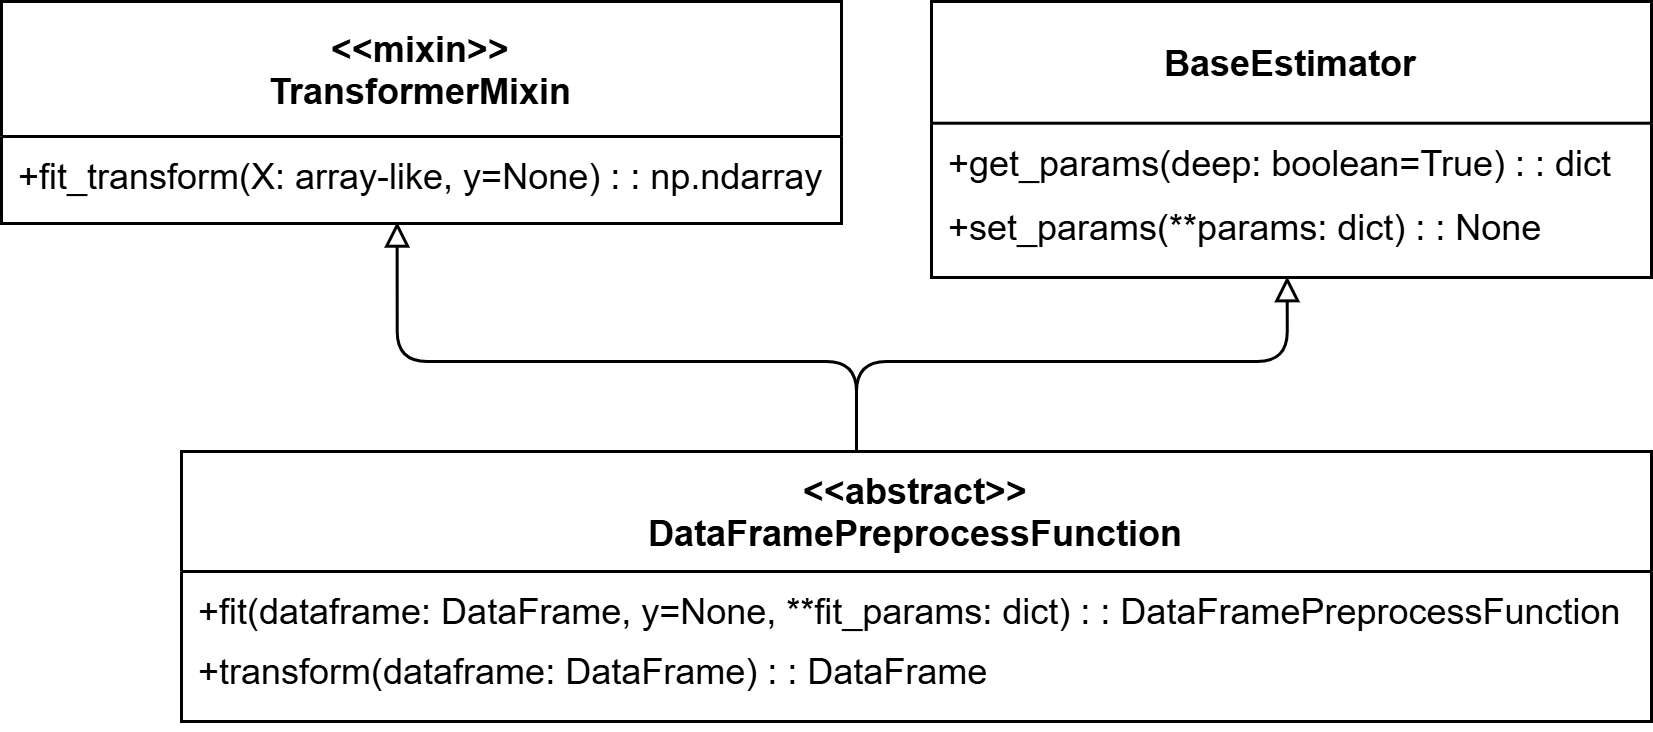
\includegraphics[scale=0.2]{figures/UML/preprocessing/dataframe_preprocess_function.png}
    \caption{Diagramma della classe \texttt{DataFramePreprocessFunction}}
\end{figure}

Tutti i \textit{transformers} della libreria estendono direttamente o indirettamente questa classe per poter implementare i metodi \texttt{fit} e \texttt{transform}. 

Vengono create anche diverse classi per poter raggruppare comportamenti comuni di alcune tipologie di \textit{transformers}:

\begin{itemize}
    \item \texttt{GroupByFunction}: estende \texttt{DataFramePreprocessFunction} e modella l'applicazione di una trasformazione su dati raggruppati (\textit{group-by}). Viene definito il metodo astratto \texttt{\_build\_transform\_function}, applicando il pattern \textit{Template Method}. Questo metodo viene invocato all'interno del metodo \texttt{fit} e restituisce una funzione, che viene salvata come attributo. Questa funzione viene poi utilizzata nel metodo \texttt{transform} sui dati in input trasformandoli.
    
    La classe viene estesa a sua volta da \texttt{Normalizer}, che normalizza vettori per lunghezza unitaria.

    \begin{figure}[H]
        \centering
        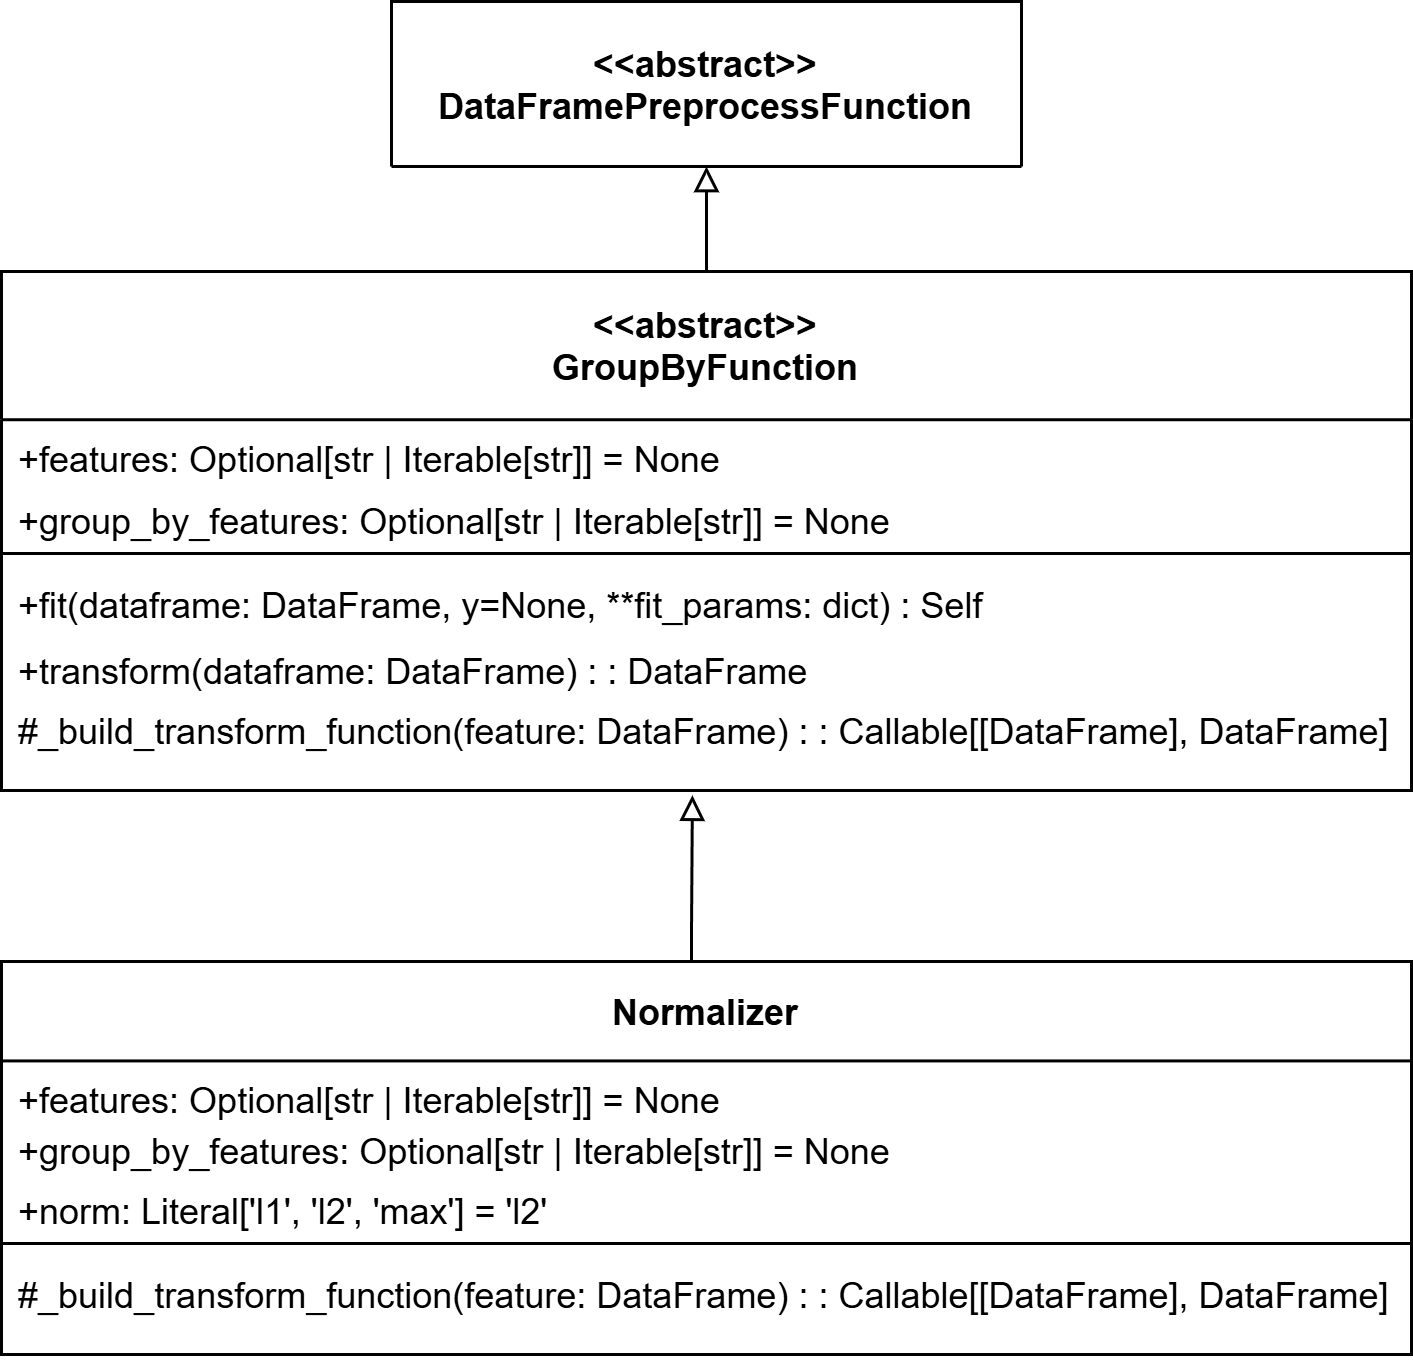
\includegraphics[scale=0.2]{figures/UML/preprocessing/group_by.png}
        \caption{Gerarchia di \texttt{GroupByFunction}}
    \end{figure}

    \item \texttt{InverseTransformer}: classe base per trasformazioni invertibili (che permettono di tornare ai dati originali) grazie alla invocazione al metodo \texttt{inverse\_transform}.
    
    La classe viene estesa a sua volta da \texttt{LabelEncoder}, che codifica etichette categoriali in valori numerici e permette l'inversione.
    
    \begin{figure}[H]
        \centering
        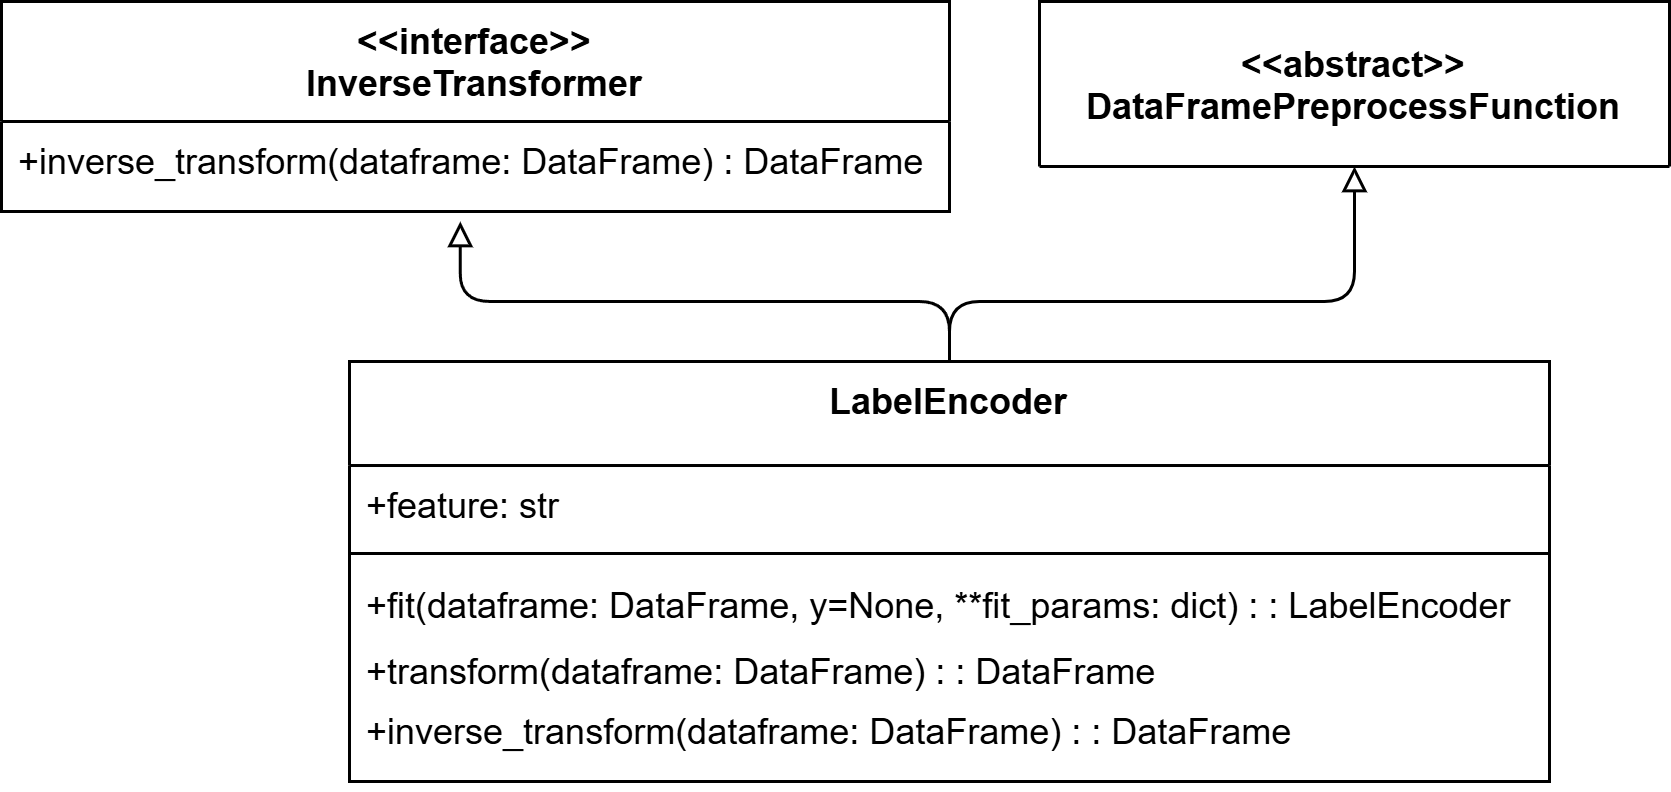
\includegraphics[scale=0.2]{figures/UML/preprocessing/inverse_transformer.png}
        \caption{Gerarchia di \texttt{InverseTransformer}}
    \end{figure}

    \item \texttt{InvertibleGroupByFunction}: estende \texttt{GroupByFunction} e \texttt{InverseTransformer}, permette di invertire le trasformazioni su gruppi. Vengono definiti i metodi astratti \texttt{\_build\_transform\_function} e \texttt{\_build\_inverse\_function}, applicando il pattern \textit{Template Method}, i quali vengono invocati entrambi dentro i metodi \texttt{fit} e restituiscono una funzione ciascuno che vengono salvate come attributi. Queste funzioni vengono poi utilizzate durante l'invocazione dei metodi \texttt{transform} e di \texttt{inverse\_transform} per applicare la trasformazione corrispondente.
    
    La classe viene estesa a sua volta da \texttt{StandardScaler}, che normalizza i dati rendendoli con media $0$ e deviazione standard $1$, e \texttt{MinMaxScaler}, che scala i dati in un intervallo specifico (di solito $[0, 1]$).
    
    \begin{figure}[H]
        \centering
        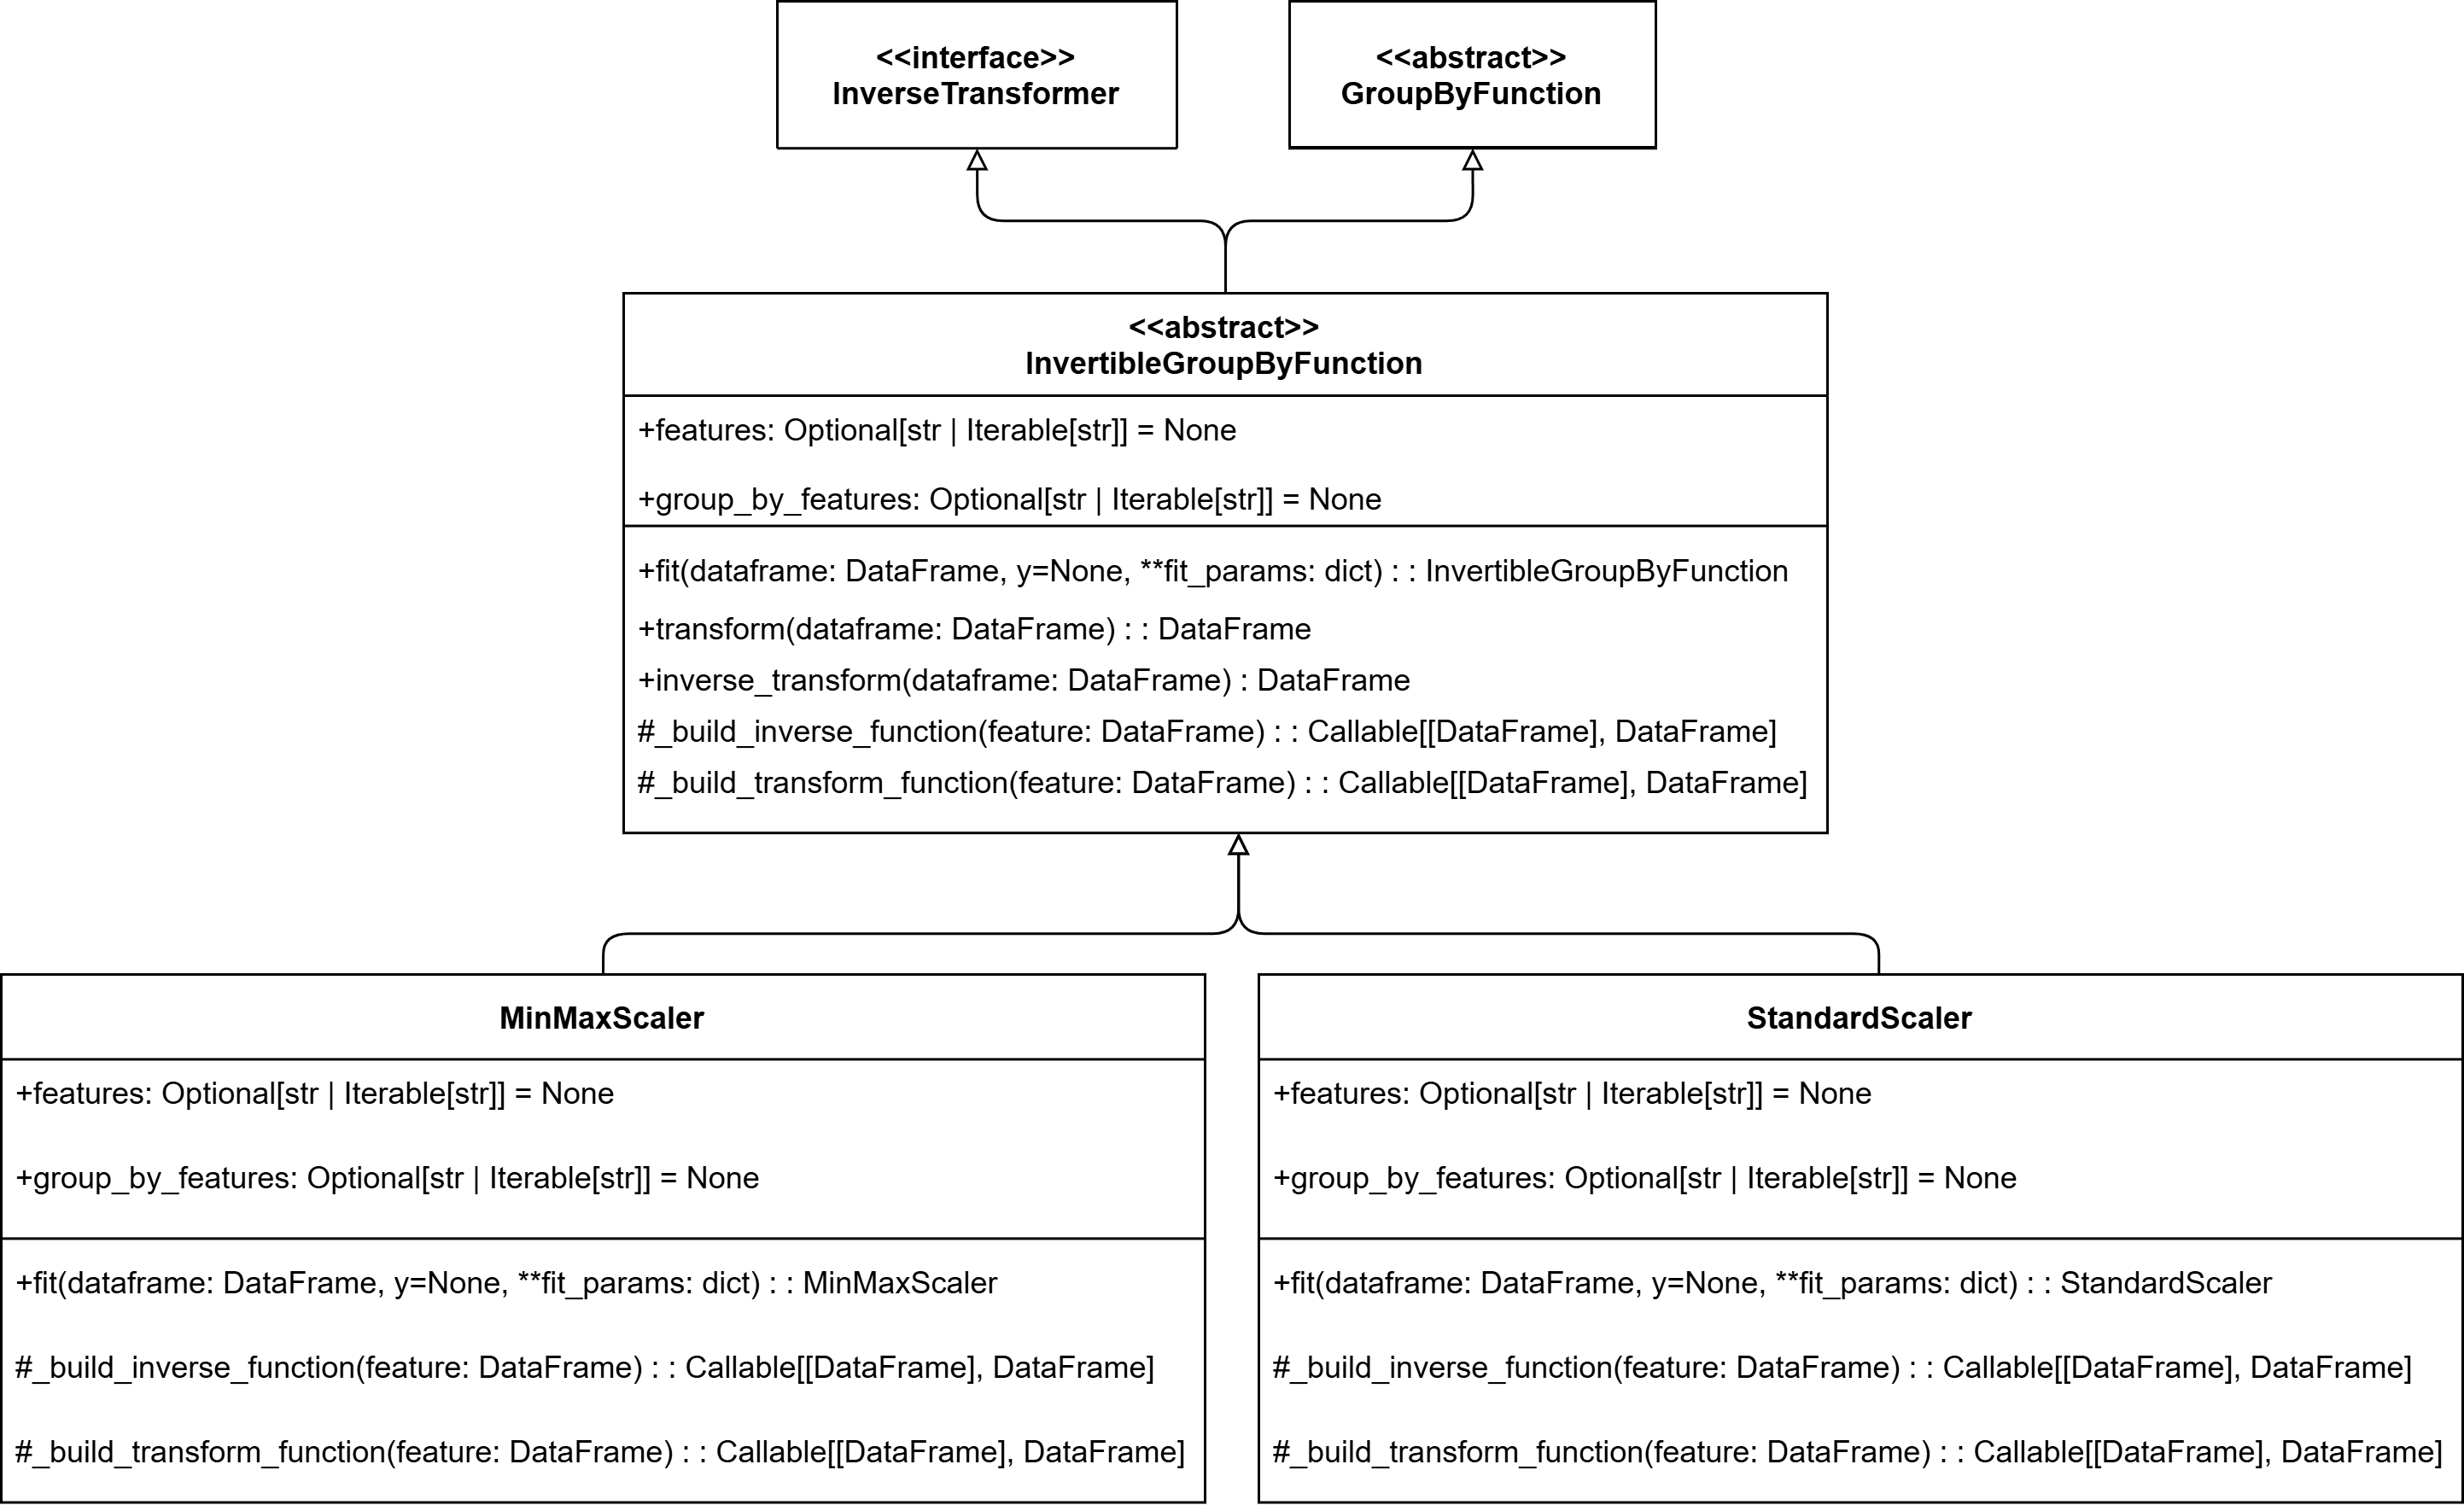
\includegraphics[scale=0.1]{figures/UML/preprocessing/invertible_group_by.png}
        \caption{Gerarchia di \texttt{InvertibleGroupByFunction}}
    \end{figure}
    
    \item \texttt{BinDensity}: estende \texttt{DataFramePreprocessFunction}, si occupa di binning e densità dei dati. Viene definito il metodo astratto \texttt{\_divide} applicando il pattern \textit{Template Method}, il quale viene invocato dentro il metodo \texttt{fit} e restituisce una funzione che viene salvata come attributo. Questa funzione viene poi utilizzata nel metodo \texttt{transform} per applicare la trasformazione corrispondente.
    
    La classe viene estesa a sua volta da \texttt{BinThreshold}, che effettua \textit{binning} basato su una soglia di frequenza, e \texttt{BinCumulative}, che effettua \textit{binning} basato su cumulativi di distribuzione.
    \begin{figure}[H]
        \centering
        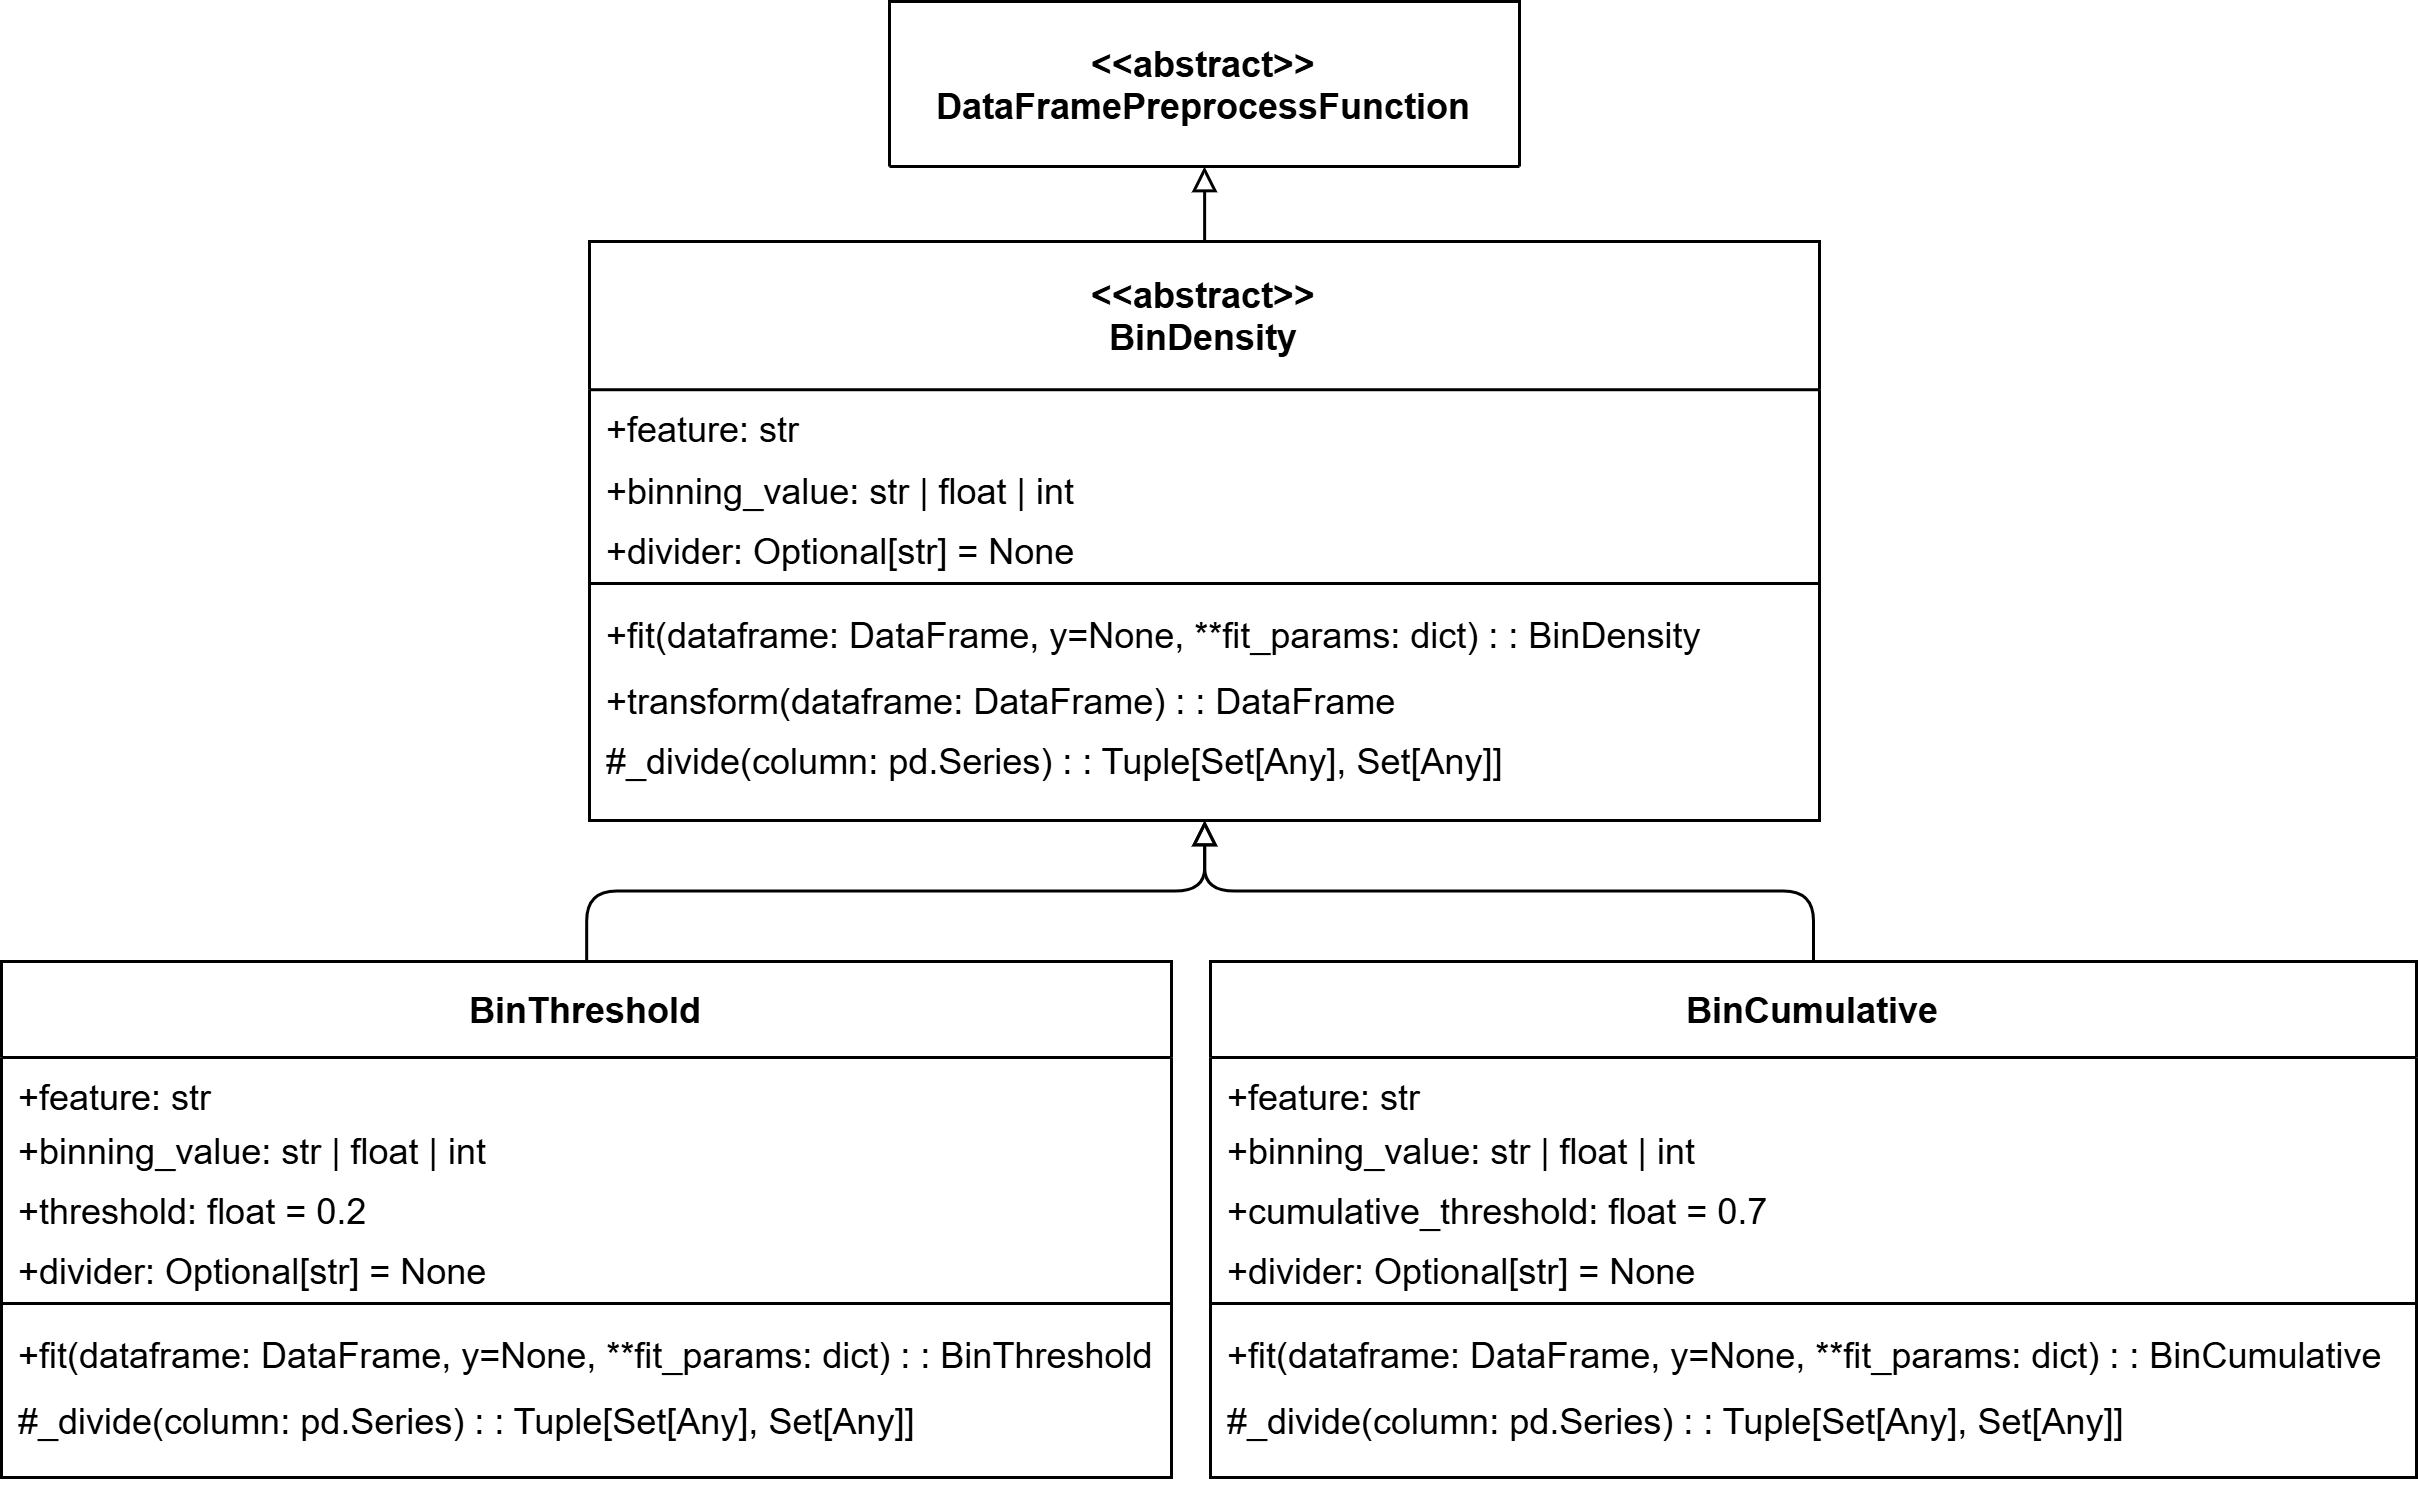
\includegraphics[scale=0.10]{figures/UML/preprocessing/bin_density.png}
        \caption{Gerarchia di \texttt{BinDensity}}
    \end{figure}
\end{itemize}

\subsection{Pipeline pattern}

Si è deciso di utilizzare il \textit{pipeline pattern} per l'applicazione dei \textit{transformer} ai dati. Questo pattern è una struttura architetturale in cui una serie di elaborazioni vengono applicate sequenzialmente a un flusso di dati, in questo caso il \textit{dataset} del tipo \textit{DataFrame}. Ogni stadio della \textit{pipeline} prende in input l'output dello stadio precedente, eseguendo una trasformazione. Ogni componente della \textit{pipeline} è modulare, indipendente, non modifica i valori in input (genera una copia in output) né causa \textit{side effect}. L'elaborazione delle trasformazioni avviene in sequenza ed è possibile modificare sia l'ordine delle trasformazioni che le trasformazioni stesse. In caso ci fosse un errore in una delle trasformazioni la \textit{pipeline} non va a buon fine.

\begin{figure}[H]
    \centering
    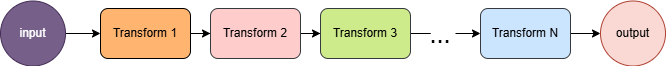
\includegraphics[scale=0.45]{figures/pipeline.png}
    \caption{\textit{Pipeline pattern}}
    \label{fig:pipeline}
\end{figure}

La pipeline, anch'essa una \textit{DataFramePreprocessFunction} che applica tutte le trasformazioni specificate, è definita come \texttt{PreprocessPipeline}.

\begin{figure}[H]
    \centering
    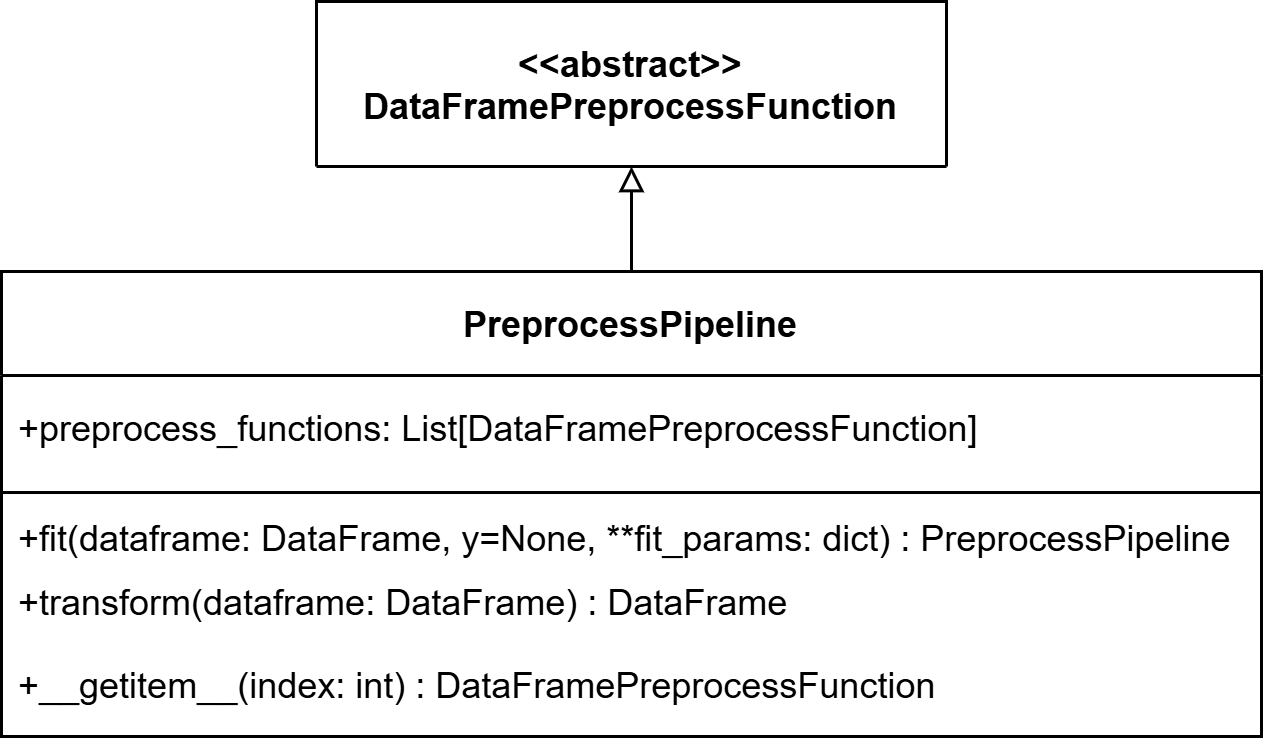
\includegraphics[scale=0.2]{figures/UML/preprocessing/preprocess_pipeline.png}
    \caption{Diagramma della classe \texttt{PreprocessPipeline}}
    \label{fig:preprocess_pipeline}
\end{figure}

Un esempio di utilizzo è:

\begin{lstlisting}[caption=esempio di utilizzo di \texttt{PreprocessPipeline}]
pipeline = PreprocessPipeline([
    Drop('timestamp'),
    Bin('rating', bins=5),
    ...
])
preprocessed_dataset = pipeline.fit_transform(dataset) 
\end{lstlisting}

\subsection{Tranformers}

Un elenco dei \textit{transformers} che estendono direttamente la classe \\
\texttt{DataFramePreprocessFunction} e una descrizione delle operazioni che svolgono:

\begin{itemize}
    \item \texttt{Select}: seleziona specifiche colonne
    \item \texttt{FillNa}: riempie i valori mancanti
    \item \texttt{Filter}: filtra le righe secondo una funzione di filtro
    \item \texttt{Drop}: rimuove colonne specificate
    \item \texttt{Rename}: rinomina colonne
    \item \texttt{Update}: aggiorna dati esistenti
    \item \texttt{Round}: arrotonda valori numerici a un numero specifico di cifre decimali
    \item \texttt{Bin}: crea categorie (\textit{bin}) da valori continui in una colonna
    \item \texttt{ExtractDate}: estrae componenti della data da una colonna \textit{datetime}
    \item \texttt{DropNa}: elimina righe con valori mancanti in colonne specifiche
    \item \texttt{DropDuplicates}: rimuove righe duplicate
    \item \texttt{Cycle}: calcola valori ciclici (es. per data o tempo)
    \item \texttt{Clip}: limita i valori numerici entro un intervallo specificato
    \item \texttt{Map}: mappa i valori di una colonna usando una funzione o dizionario
    \item \texttt{OneHotEncode}: codifica variabili categoriali in variabili \textit{dummy} (\textit{one-hot})
    \item \texttt{Condense}: aggrega dati raggruppandoli e concatenandoli
    \item \texttt{ToCOOMatrix}: trasforma dati in una matrice sparsa in rappresentazione \textit{COO} (sempre nel tipo \textit{DataFrame})
\end{itemize}

\begin{figure}[H]
    \centering
    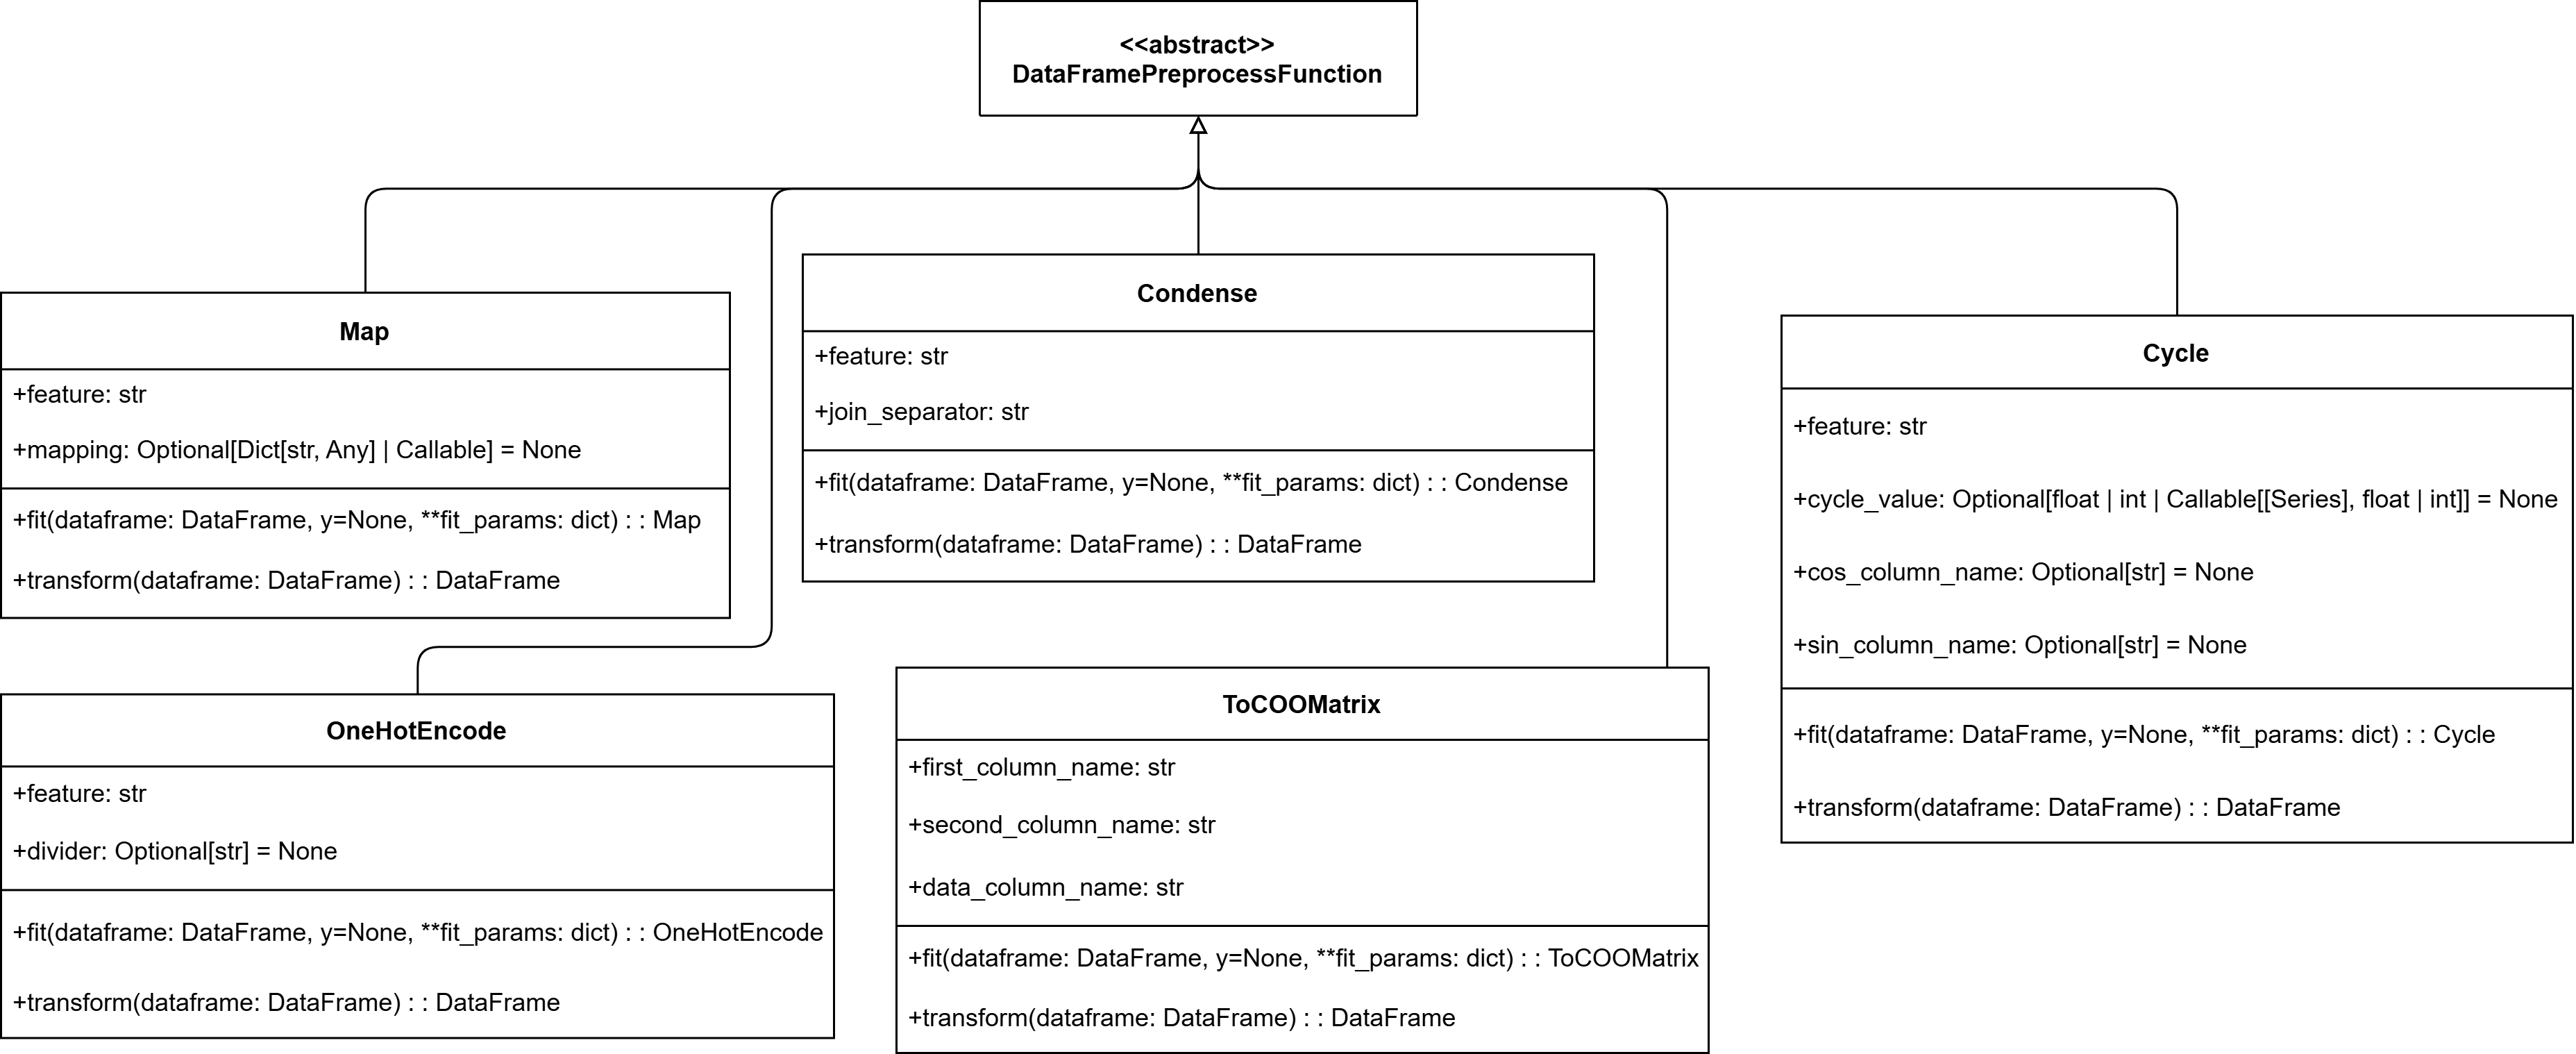
\includegraphics[angle=90, scale=0.14]{figures/UML/preprocessing/direct_1.png}
    \caption{Diagrammi delle classi \texttt{Map}, \texttt{Condense}, \texttt{Cycle}, \\ \texttt{OneHotEncode}, \texttt{ToCOOMatrix}}

\end{figure}\begin{figure}[H]
    \centering
    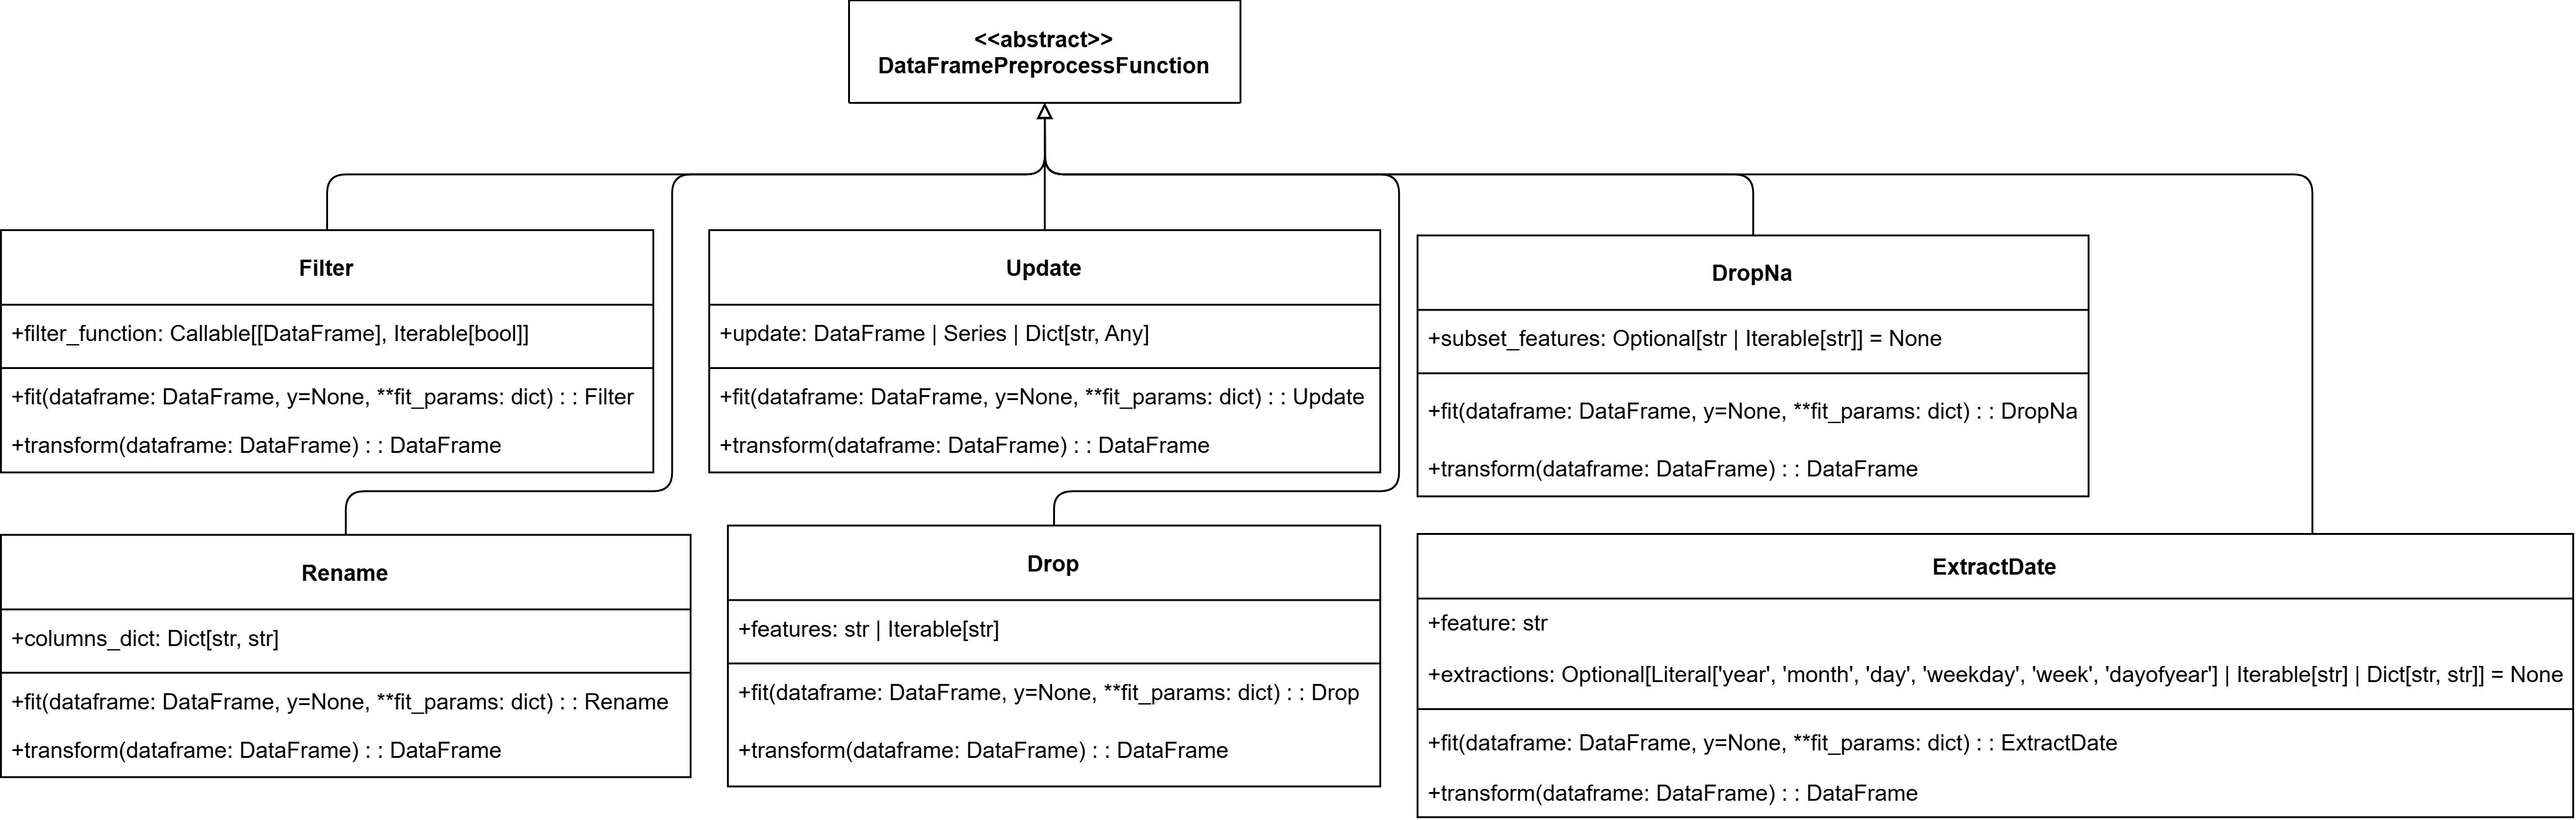
\includegraphics[angle=90, scale=0.13]{figures/UML/preprocessing/direct_2.png}
    \caption{Diagrammi delle classi \texttt{Filter}, \texttt{Update}, \texttt{DropNa}, \texttt{Rename}, \texttt{Drop}, \texttt{ExtractDate}}

\end{figure}\begin{figure}[H]
    \centering
    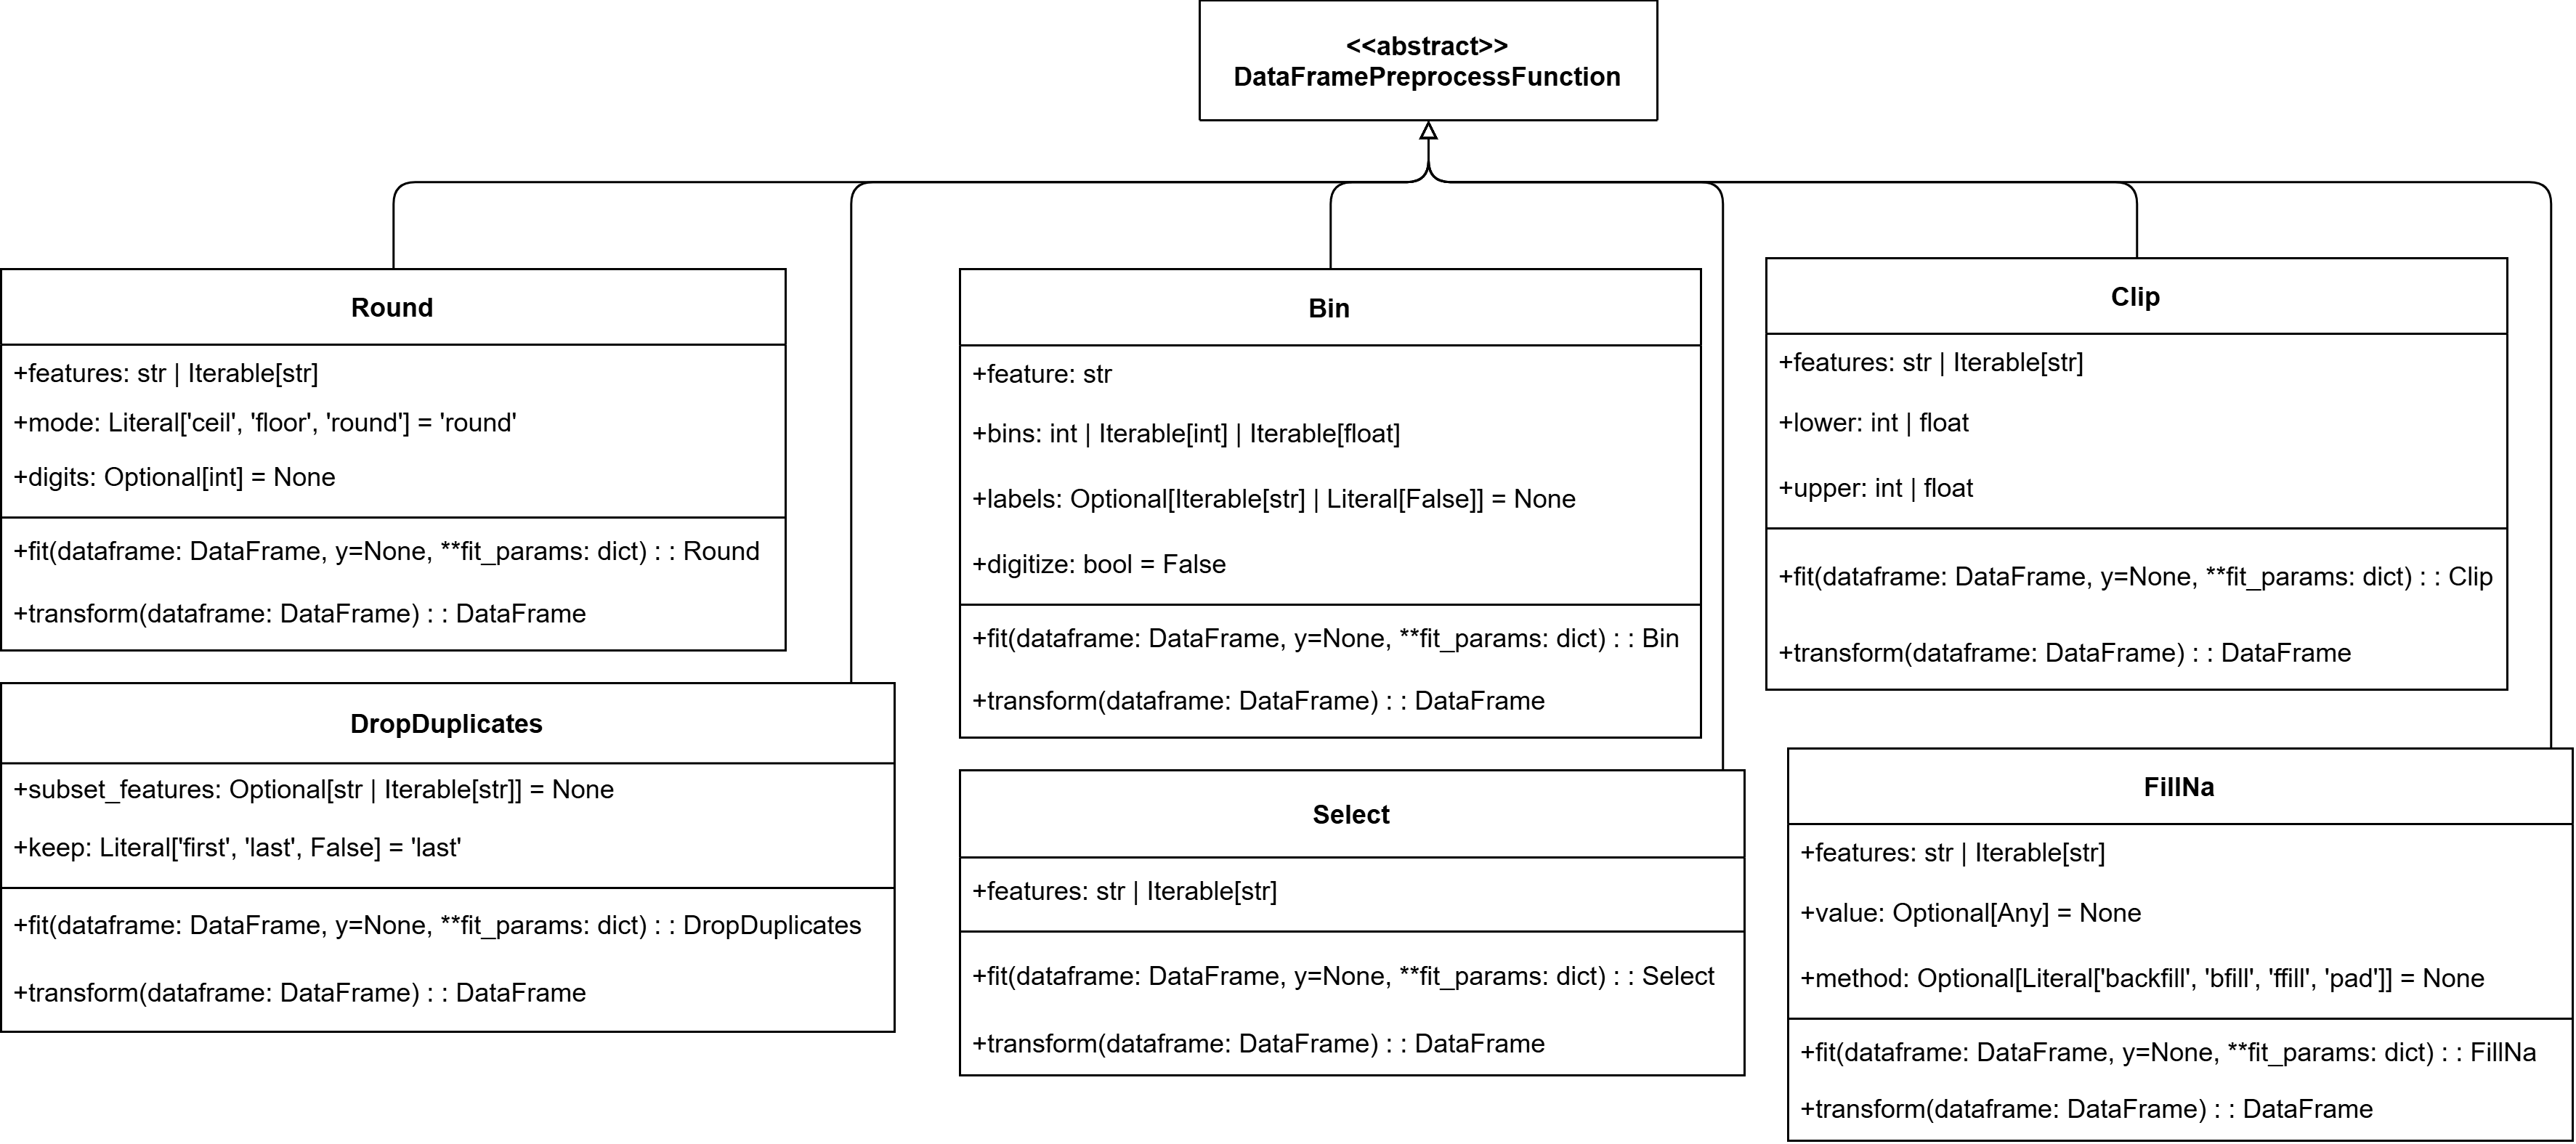
\includegraphics[angle=90, scale=0.15]{figures/UML/preprocessing/direct_3.png}
    \caption{Diagrammi delle classi \texttt{Round}, \texttt{Bin}, \texttt{Clip}, \texttt{DropDuplicates}, \texttt{Select}, \texttt{FillNa}}
\end{figure}

\section{Models}
Il modulo comprende l'insieme delle classi dei modelli di \textit{recommendation}.

Per i modelli che gestiscono feedback espliciti sono presenti i seguenti algoritmi:

\begin{itemize}
    \item \textit{SVD}~\ref{svd}
    \item \textit{SVD++}~\ref{svdpp}
    \item \textit{NFM}~\ref{nmf}
    \item \textit{KNN con baseline}~\ref{knn}
    \item \textit{CoClustering}~\ref{coclustering}
    \item \textit{SlopeOne}~\ref{slopeone}
\end{itemize}

mentre per quelli che gestiscono feedback impliciti:

\begin{itemize}
    \item \textit{ALS}~\ref{als} 
    \item \textit{BRP}~\ref{bpr} 
    \item \textit{LMF}~\ref{lmf}
    \item \textit{LightFM}~\ref{lightfm}  
\end{itemize}

Per ogni algoritmo, la libreria applica il pattern \textit{Adapter} per rendere compatibili i modelli con la libreria \textit{Scikit-learn}.

\subsection{Compatibilità con Scikit-learn dei modelli}\label{compatibilita_sklearn}

Per definire un modello custom compatibile con la suite di \textit{Scikit-learn} occorre seguire alcuni requisiti che possono essere variabili. Vengono presentate le scelte effettuate per la libreria e che ogni modello deve rispettare:

\begin{itemize}
    \item estendere la classe \texttt{BaseEstimator}
    \item implementare il metodo \texttt{fit} che abbia almeno come parametri:
    \begin{itemize}
        \item \texttt{X} di tipo \textit{array-like}, \textit{sparse matrix} o \textit{DataFrame}
        \item \texttt{y} che in questo caso viene sempre inizializzata con un valore di default \texttt{None} e che non viene utilizzata ma che viene specificata per convenzione per avere una API coerente
    \end{itemize}
    \item implementare il metodo \texttt{predict} che abbia almeno come parametro X di tipo \textit{array-like}, \textit{sparse matrix} o \textit{DataFrame} e che restituisca come risultato un \textit{NumPy array}
    \item tutti i campi devono essere pubblici e chiamarsi allo stesso modo dei parametri del costruttore
    \item non ci devono essere computazioni all'interno del costruttore ma solamente le inizializzazioni dei campi
    \item una volta che il metodo \texttt{fit} viene invocato devono essere valorizzati parametri che terminano con il carattere "\_" (e.g. \texttt{model.item\_factors\_} e \\ \texttt{model.user\_factors\_})
    \item inserire, all'interno del metodo \texttt{predict}, un controllo che verifichi che il modello sia stato addestrato, utilizzando la funzione \texttt{check\_is\_fitted}. Questa funzione verifica la presenza di almeno un attributo il cui nome termini con il carattere ``\_'' (convenzionalmente utilizzato da \textit{Scikit-learn} per indicare che l'attributo è stato appreso durante il training). In caso contrario, viene sollevata un'eccezione di tipo \texttt{NotFittedError}
\end{itemize}

I modelli possono, in base alle necessità, aggiungere parametri aggiuntivi alle funzioni di \texttt{fit} e di \texttt{predict}, per esempio eventuali \texttt{user\_features} o \texttt{item\_features}.

\subsection{Salvataggio modelli}

Viene definita l'interfaccia \texttt{PersistableModel} che espone il metodo \texttt{save} per il salvataggio dei modelli. Il metodo riceve come parametro \texttt{fileobj\_or\_path} che corrisponde al nome del file (che include anche il percorso, tipo \texttt{str}) oppure un oggetto file aperto (tipo \texttt{io.IOBase}) su cui salvare il modello.

\begin{figure}[H]
    \centering
    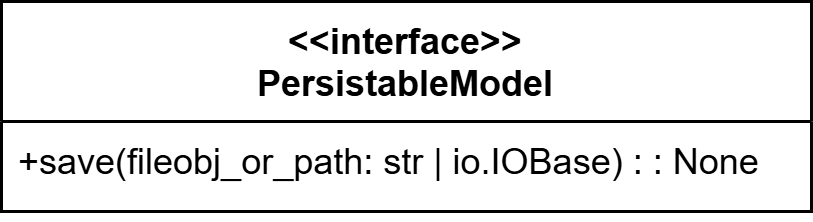
\includegraphics[scale=0.3]{figures/UML/models/persistable_model.png}
    \caption{Diagramma del'interfaccia \texttt{PersistableModel}}
\end{figure}

Per il caricamento da file ogni modello implementerà autonomamente un metodo \texttt{load}, che potrà essere tipo \textit{classmethod} oppure un \textit{staticmethod}.

\subsection{Model fit data}\label{model_fit_data}

I vari modelli possono essere addestrati con il metodo \texttt{fit} su diversi formati di dati, purché rispettino i vincoli sopra descritti. Per i modelli sviluppati si è deciso un formato standard. La prima colonna è composta dagli \textit{user\_id}, che corrispondono agli id degli \textit{user}, la seconda colonna all'\textit{item\_id}, che corrispondono agli id degli \textit{item}, e le eventuali colonne successive a informazioni aggiuntive sull'interazione, per esempio il \textit{rating} o il \textit{timestamp}. Le uniche informazioni obbligatorie sono quindi solamente le coppie (\textit{user\_id}, \textit{item\_id}). I modelli possono in modo indipendente introdurre eventuali vincoli sui dati in input.

Un esempio di input in formato \textit{DataFrame}:

\begin{table}[H]
    \centering
    \begin{tabular}{|c|c|c|c|}
    \hline
    \textbf{user\_id} & \textbf{item\_id} & \textbf{rating} & \textbf{timestamp} \\
    \hline
        101 & 501 & 4.0 & 2021-03-14 08:23:45 \\
        102 & 502 & 5.0 & 2022-07-19 16:45:10 \\
        103 & 503 & 3.5 & 2020-11-03 03:12:00 \\
        104 & 504 & 2.0 & 2019-01-27 22:58:36 \\
        105 & 505 & 4.5 & 2023-09-05 13:37:21 \\
    \hline
    \end{tabular}
    \caption{Esempio di input con due colonne extra per i \textit{rating} e il \textit{timestamp}}
    \label{tab:ratings}
\end{table}

\subsubsection{Ids}

Ogni volta che si fa riferimento ad un id, che sia \texttt{user\_id} o \texttt{item\_id}, si considera che il tipo sia \texttt{int} oppure \texttt{str}. 

\subsection{Model predict data}\label{model_predict_data}

I vari modelli possono predire il \textit{rating} o lo \textit{score} con il metodo \texttt{predict} su diversi formati di dati, purché rispettino i vincoli sopra descritti. Il formato standard deciso è identico a quello utilizzato per l'addestramento~\ref{model_fit_data}. I modelli possono in modo indipendente introdurre eventuali vincoli sui dati in input.

In questo caso però il modello utilizza la singola coppia (\textit{user\_id}, \textit{item\_id}) alla quale viene associato un \textit{rating} o lo \textit{score} in base al tipo di modello utilizzato, rispettivamente per feedback espliciti e per feedback impliciti. Se, per esempio, vengono dati in input al modello, che gestisce feedback impliciti, cinque coppie (\textit{user\_id}, \textit{item\_id}) quest'ultimo restituisce un \textit{NumPy array} di cinque valori, ciascuno corrispondente allo \textit{score} ottenuto da ciascuna coppia. Se si vuole ottenere il \textit{ranking} occorre ordinare gli \textit{score} ottenuti in ordine decrescente. Se si vuole calcolare \textit{rating} o lo \textit{score}, dati un insieme $U$ di \textit{user} e $I$ di \textit{item}, occorre dare in input al metodo \texttt{predict} tutte le combinazioni $\left\{(u, i) \mid u \in U,\; i \in I \right\}$.

Un esempio di input in formato \textit{DataFrame} e di output in formato \textit{NumPy array}:

\begin{table}[H]
    \centering
    \begin{minipage}{0.6\textwidth}
        \centering
        \begin{tabular}{|c|c|c|c|}
        \hline
        \textbf{user\_id} & \textbf{item\_id} \\
        \hline
            101 & 501 \\
            102 & 502 \\
            103 & 503 \\
            104 & 504 \\
            105 & 505 \\
        \hline
        \end{tabular}
    \end{minipage}%
    \hfill
    \begin{minipage}{0.3\textwidth}
        \centering
        \begin{tabular}{|c|}
        \hline
        0.97 \\
        -0.12 \\
        1.02 \\
        0.08 \\
        0.55 \\
        \hline
        \end{tabular}
    \end{minipage}
    \caption{Esempio output restituito dal modello che gestisce feedback impliciti}
    \label{tab:ratings_with_score}
\end{table}

Importante considerare che gli \textit{score}, generati dai modelli impliciti, singolarmente non hanno alcun significato ma vengono utilizzati solamente per definire un ordinamento.

\subsection{Similarità user-user o item-item}

I modelli posso estendere l'interfaccia \texttt{SimilarityModel} che espone due metodi per calcolare la similarità tra \textit{users-users} e tra \textit{items-items}. Solitamente il calcolo include l'utilizzo di vettori \textit{embedding} appresi durante l'addestramento. Sono strumento che permette di effettuare \textit{up-selling}, trovando \textit{item} simili si può proporre una versione più costosa o avanzata.

Il metodo \texttt{similar\_users} ha i seguenti parametri:

\begin{itemize}
    \item \texttt{user\_id} (singolo id o \texttt{NumPy array} o \texttt{Series}): id dello \textit{user} o lista di id per cui si desidera trovare \textit{user} simili
    \item \texttt{N} (\texttt{int}): numero di \textit{user} simili da restituire. Il valore di default è 10
    \item \texttt{filter\_users} (\texttt{NumPy array} o \texttt{Series}): lista di id di \textit{user} da escludere dai risultati
    \item \texttt{users} (\texttt{NumPy array} o \texttt{Series}): lista di id di \textit{users} da includere nei risultati. Non può essere utilizzata insieme a \texttt{filter\_users}
\end{itemize}

Il metodo \texttt{similar\_items} ha i seguenti parametri:
\begin{itemize}
    \item \texttt{item\_id} (singolo id o \texttt{NumPy array} o \texttt{Series}): id dell'\textit{item} o lista di id per cui si desidera trovare \textit{item} simili
    \item \texttt{N} (\texttt{int}): numero di \textit{item} simili da restituire. Il valore di default è 10
    \item \texttt{filter\_items} (\texttt{NumPy array} o \texttt{Series}): lista di id di \textit{item} da escludere dai risultati
    \item \texttt{items} (\texttt{NumPy array} o \texttt{Series}): lista di id di \textit{item} da includere nei risultati. Non può essere utilizzata insieme a \texttt{filter\_items}
\end{itemize}

Entrambi i metodo restituiscono un \textit{NumPy array} di (\textit{user\_id}/\textit{item\_id}, \textit{score}), dove lo \textit{score} indica quanto sono simili. In base al modello utilizzato il valore potrebbe essere compreso in un intervallo oppure no.

\begin{figure}[H]
    \centering
    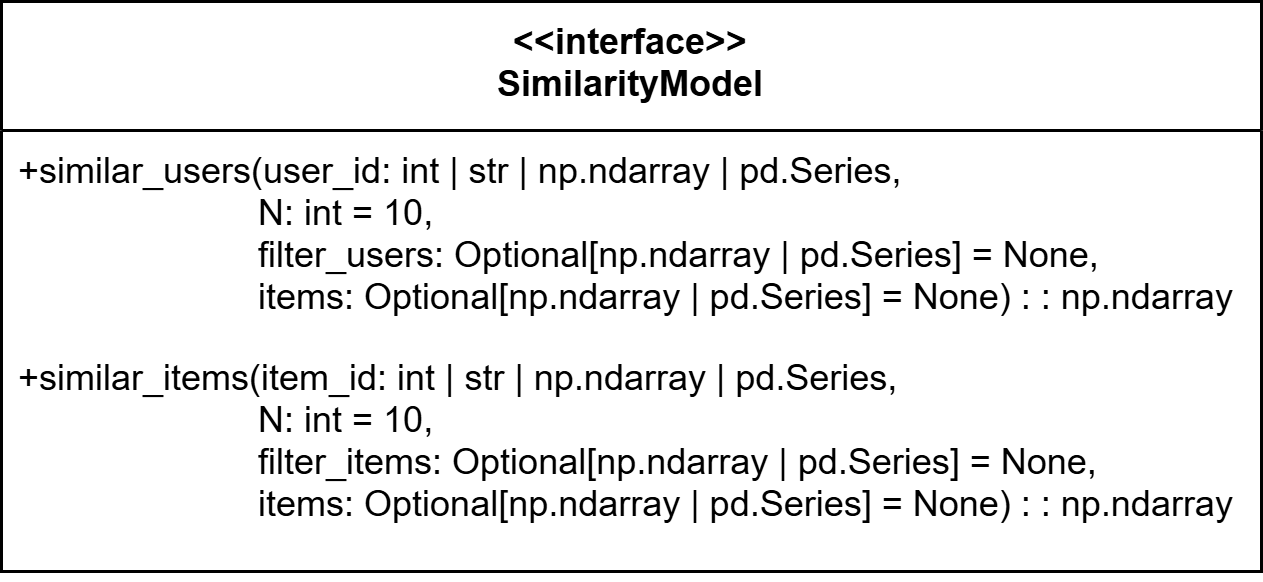
\includegraphics[scale=0.25]{figures/UML/models/similarity_model.png}
    \caption{Diagramma dell'interfaccia \texttt{SimilarityModel}}
\end{figure}

Importante inserire, all'interno del due metodi, un controllo che verifichi che il modello sia stato addestrato, utilizzando la funzione \texttt{check\_is\_fitted} come per il metodo \texttt{predict}~\ref{compatibilita_sklearn}.

\subsection{Modelli Surprise}

Viene definita la classe astratta \texttt{SurpriseModel} che estende \texttt{BaseEstimator} e \texttt{PersistableModel} e che gestisce il comportamento comune della \texttt{fit} e della \texttt{predict} di tutti i modelli della libreria \textit{Surprise}. Viene definito il metodo astratto \texttt{\_fit\_surprise\_model}, applicando il pattern \textit{Template Method}. Così facendo, l'implementazione di ogni modello deve definire solamente le modalità di addestramento del modello della libreria \textit{Surprise} e quali attributi, il cui nome termina con il carattere "\_", vengono appresi.

\begin{figure}[H]
    \centering
    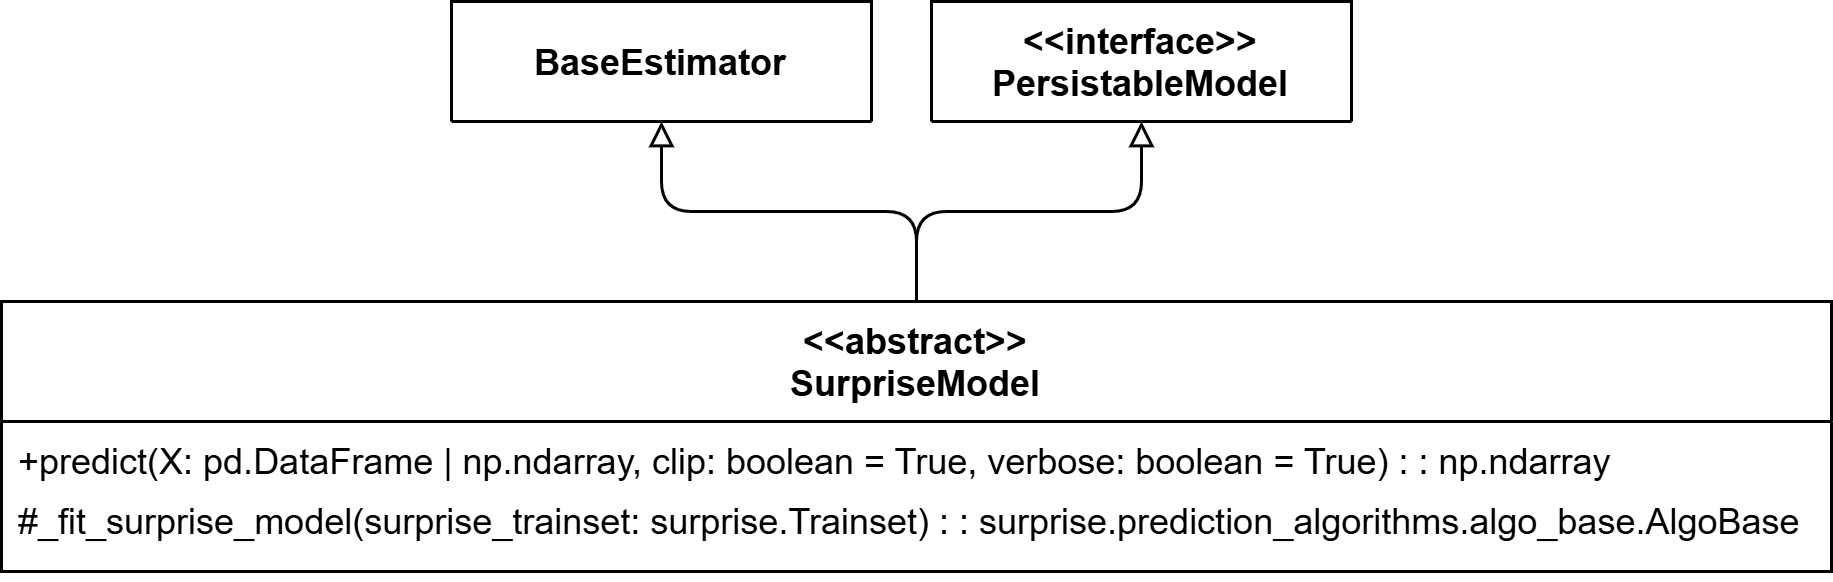
\includegraphics[scale=0.17]{figures/UML/models/surprise_model.png}
    \caption{Diagramma della classe astratta \texttt{SurpriseModel}}
\end{figure}


La classe viene estesa creando i vari adapter dei modelli:

\begin{itemize}
    \item \texttt{SVD}
    \item \texttt{SVDpp}
    \item \texttt{KNNBaseline}
    \item \texttt{SlopeOne}
    \item \texttt{CoClustering}
\end{itemize}

Ogni modello riceve nel costruttore gli stessi parametri del modello originale della libreria \textit{Surprise}.

Tutti i modelli sopra elencati gestiscono feedback espliciti e quindi i valori restituiti dal metodo \textit{predict} corrispondono a \textit{score}.


\begin{figure}[H]
    \centering
    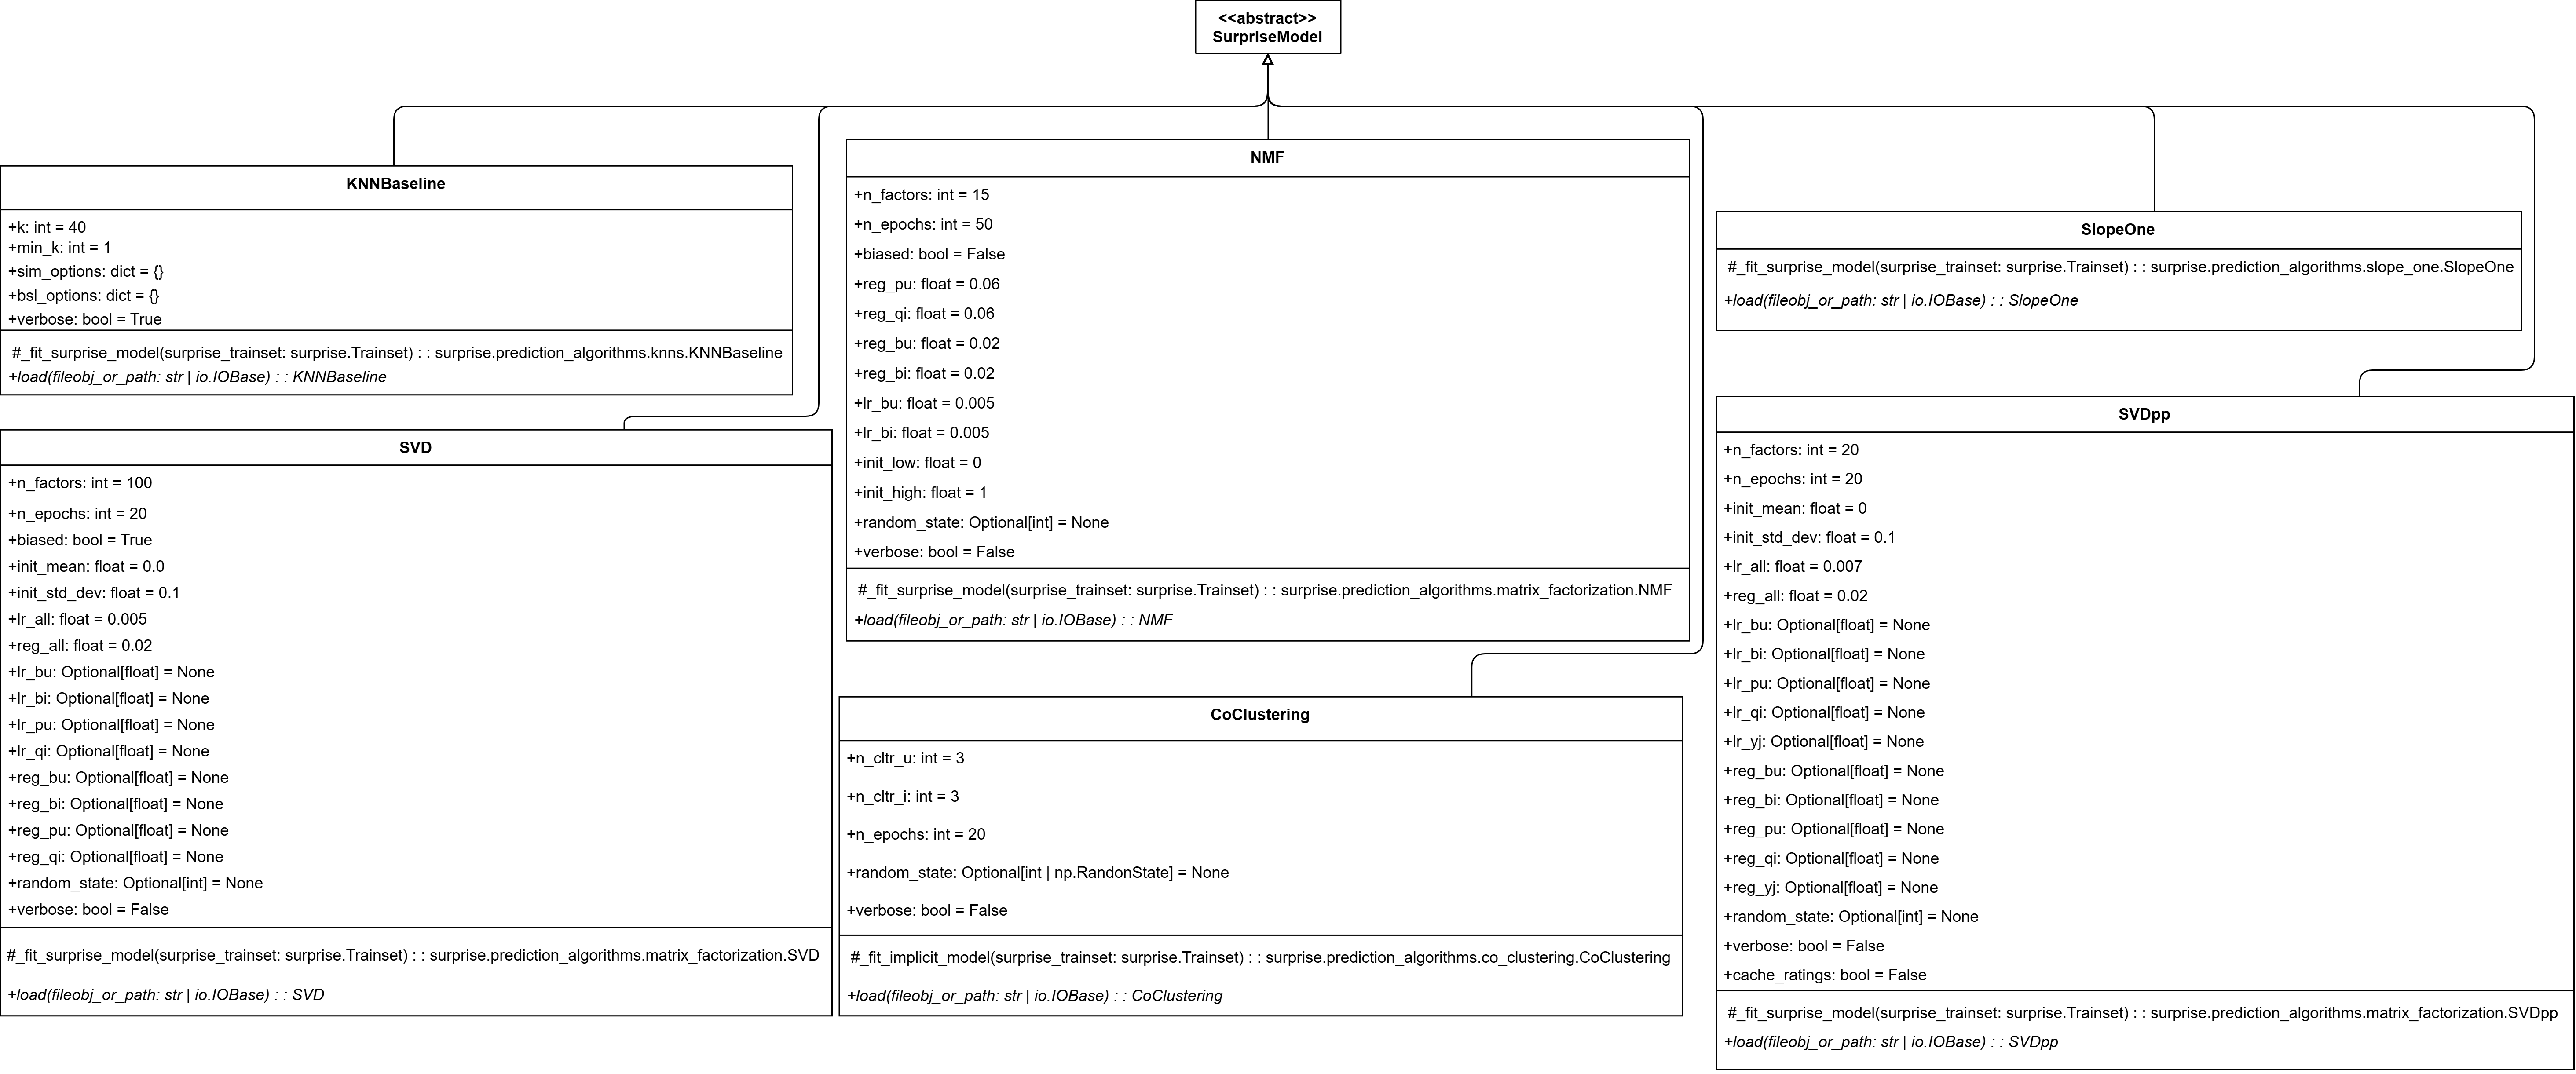
\includegraphics[angle=90, scale=0.09]{figures/UML/models/surprise_models.png}
    \caption{Diagrammi dei modelli di \textit{Surprise}}
\end{figure}

\subsubsection{Modifiche ai metodi}

Il metodo \texttt{predict} di questi modelli può riceve due parametri extra:

\begin{itemize}
    \item \texttt{clip} (\texttt{boolean}): indica se limitare la stima all'interno della scala di valutazione. Ad esempio, se $\hat{r}_{ui} = 5.5$ mentre la scala di valutazione è $[1, 5],$ allora $\hat{r}_{ui}$ viene impostato a 5. Lo stesso vale se $\hat{r}_{ui} < 1.$ Il valore di default è \texttt{True}
    \item \texttt{verbose} (\texttt{boolean}): indica se stampare i dettagli della previsione. Il valore di default è \texttt{False}
\end{itemize}

\subsection{Modelli Implicit}

Viene definita la classe astratta \texttt{ImplicitModel} che estende \texttt{BaseModel},\\ \texttt{PersistableModel} e \texttt{SimilarityModel} e che gestisce il comportamento comune della \texttt{fit} e della \texttt{predict} di tutti i modelli della libreria \textit{Implicit}. Viene definito il metodo astratto \texttt{\_fit\_implicit\_model}, applicando il pattern \textit{Template Method}. Così facendo, l'implementazione di ogni modello deve definire solamente le modalità di addestramento del modello della libreria \textit{Implicit} e quali attributi, il cui nome termina con il carattere "\_", vengono appresi.

Se il \textit{trainset} contiene una terza colonna, che deve essere numerica, questa viene considerata durante l'addestramento come il peso dell'interazione della coppia (\textit{user}, \textit{item}) (e.g. il numero di click o quante volte quel film è stato visionato). 

\begin{figure}[H]
    \centering
    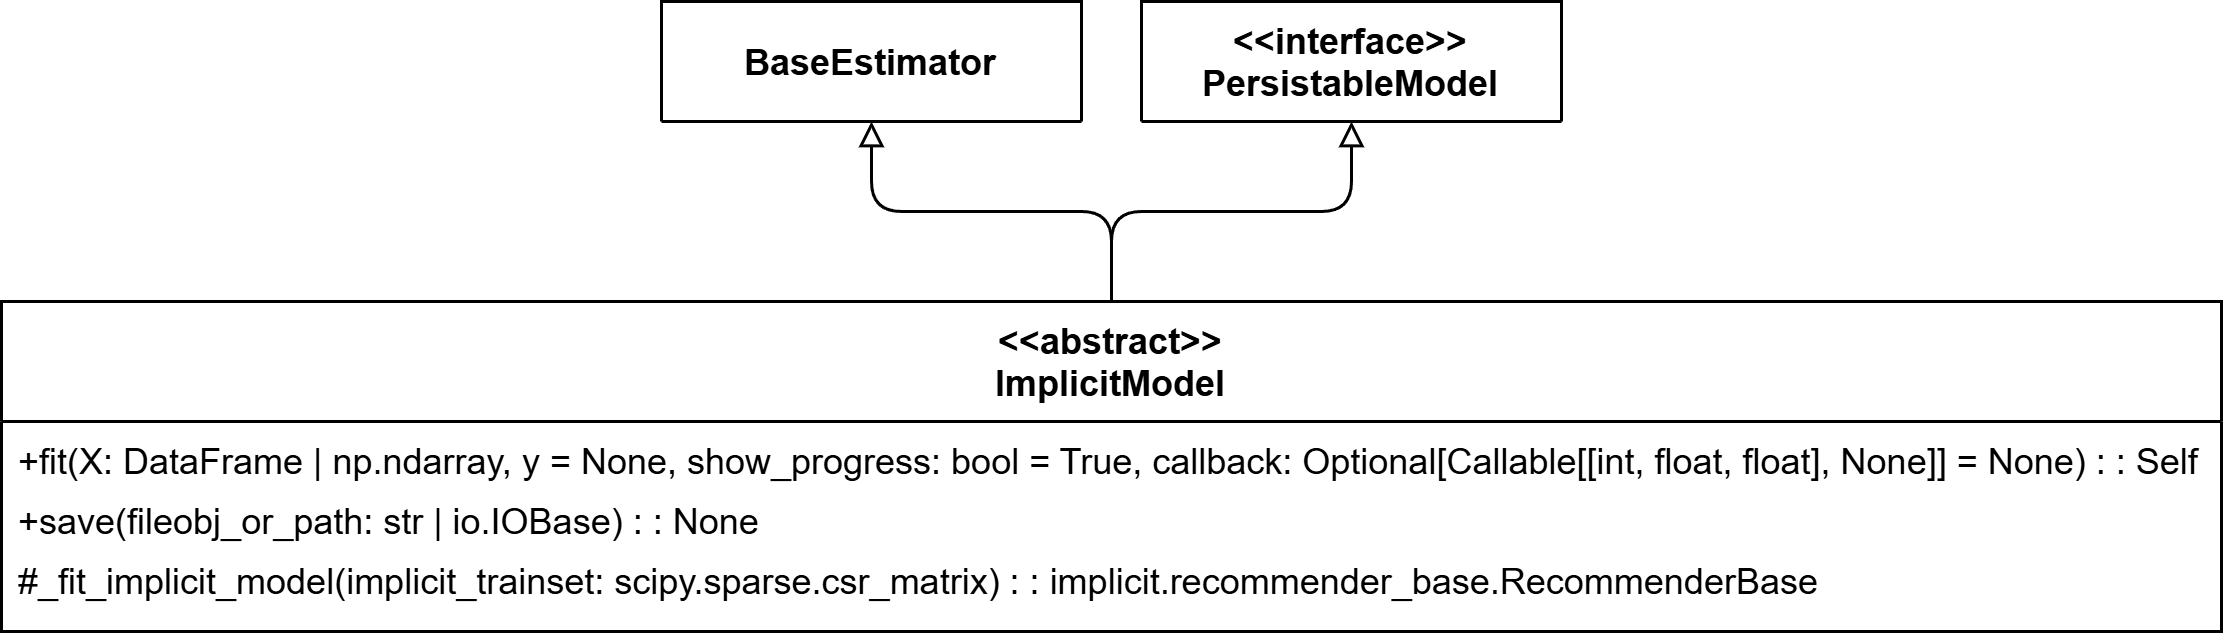
\includegraphics[scale=0.15]{figures/UML/models/implicit_model.png}
    \caption{Diagramma della classe astratta \texttt{ImplicitModel}}
\end{figure}

La classe viene estesa creando i vari adapter dei modelli:

\begin{itemize}
    \item \texttt{ALS}
    \item \texttt{BRP}
    \item \texttt{LMF}
\end{itemize}

Ogni modello riceve nel costruttore gli stessi parametri del modello originale della libreria \textit{Implicit}.

Tutti i modelli sopra elencati gestiscono feedback impliciti e quindi i valori restituiti dal metodo \textit{predict} corrispondono a \textit{rating}.

\begin{figure}[H]
    \centering
    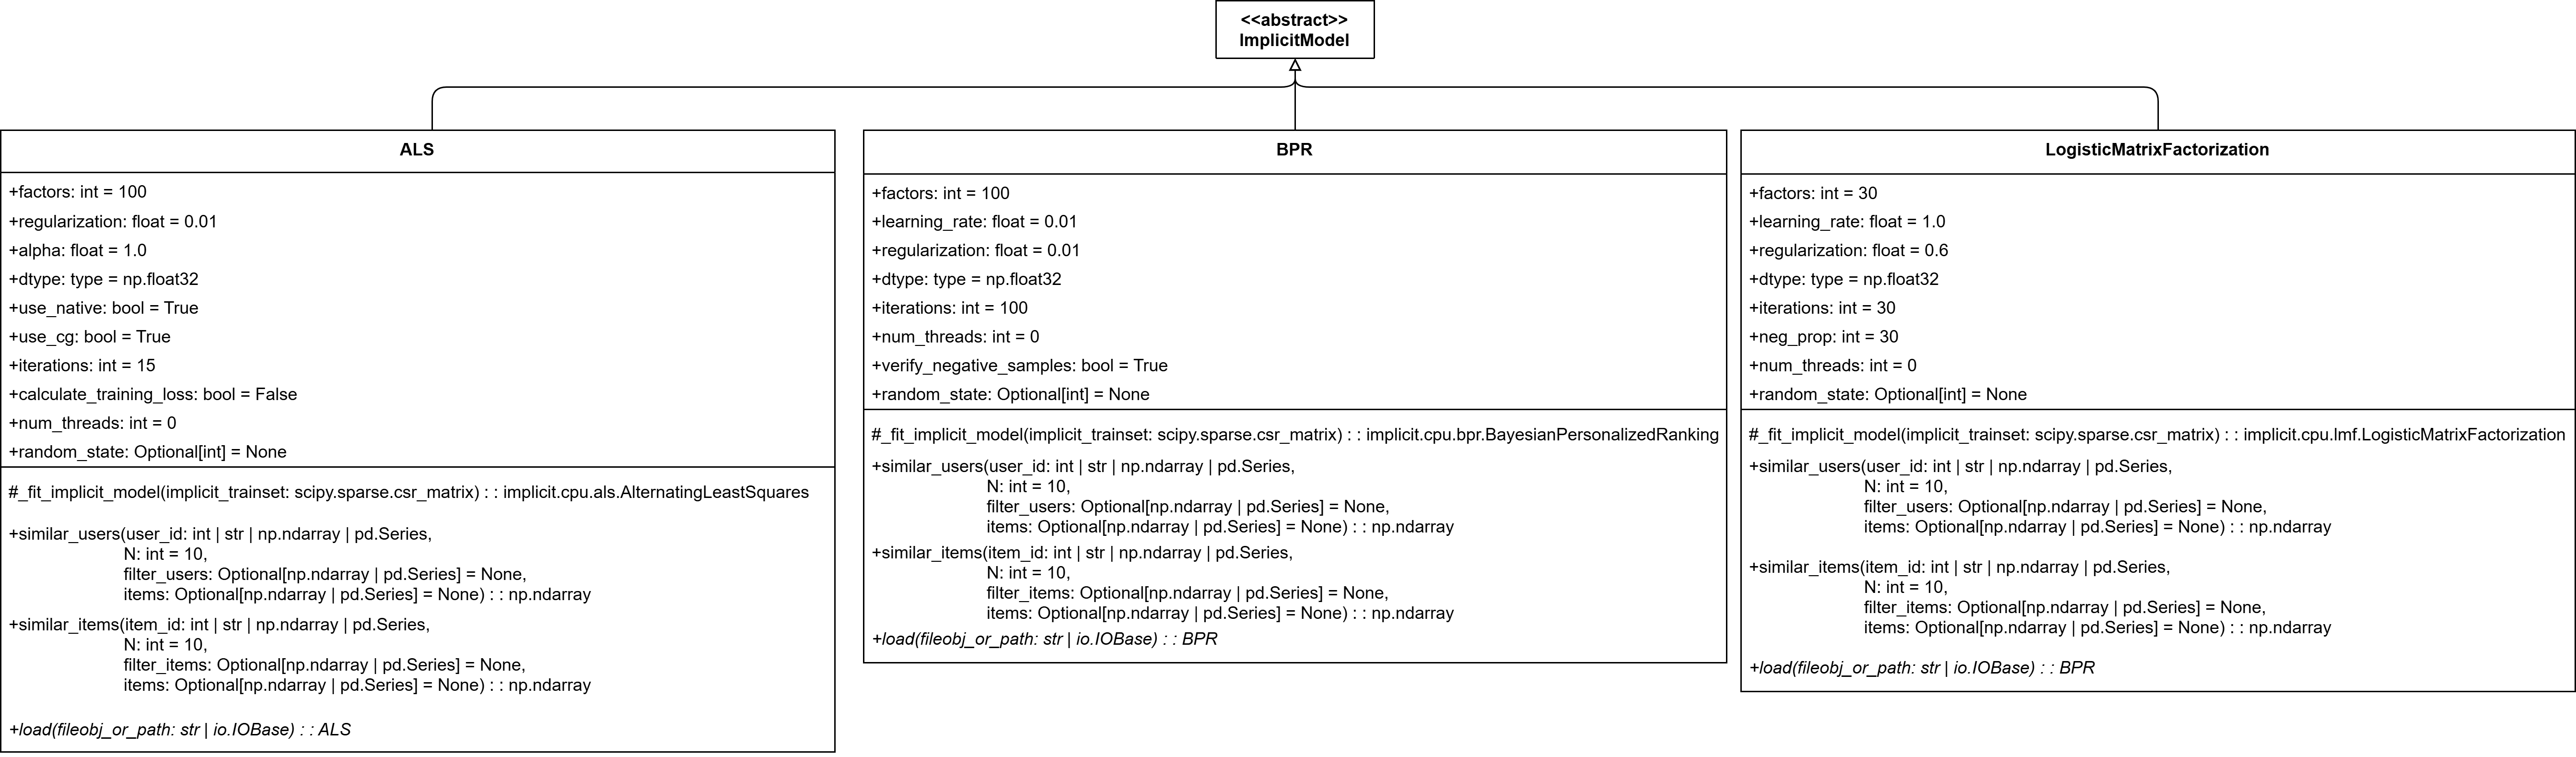
\includegraphics[angle=90, scale=0.1]{figures/UML/models/implicit_models.png}
    \caption{Diagrammi dei modelli di \textit{Implicit}}
\end{figure}

\subsubsection{Modifiche ai metodi}

Il metodo \texttt{fit} di questi modelli può riceve due parametri extra:

\begin{itemize}
    \item \texttt{show\_progress} (\texttt{bool}): indica se mostrare una barra di avanzamento durante il fitting. Il valore di default è \texttt{True}.
    \item \texttt{callback} (\texttt{Callable[[int, float, float], None]}, opzionale): funzione che viene chiamata ad ogni epoca:
    \begin{itemize}
        \item il primo parametro, di tipo \texttt{int}, corrisponde il numero corrente dell'epoca (ad esempio 1, 2, 3, \ldots)
        \item il secondo parametro, di tipo \texttt{float}, corrisponde al tempo trascorso dall'inizio dell'allenamento (in secondi, tipo \texttt{float})
        \item il terzo parametro, di tipo \texttt{float}, corrisponde alla frazione tra 0 e 1 che indica il progresso complessivo
    \end{itemize}
    Il valore di default è \texttt{None}.
\end{itemize}

\subsection{Modello LightFM}
Viene definita la classe \texttt{LightFM}, classe che estende \texttt{BaseModel}, \texttt{PersistableModel} e \texttt{SimilarityModel} e rappresenta l'\textit{Adapter} del modello \texttt{LightFM} dell'omonima libreria \texttt{LightFM}. 

Il modello gestisce feedback impliciti e quindi i valori restituiti dal metodo \textit{predict} corrispondono a \textit{score}.

Se il \textit{trainset} contiene una terza colonna, che deve essere numerica, questa viene considerata durante l'addestramento come il peso dell'interazione della coppia (\textit{user}, \textit{item}) (e.g. il numero di click o quante volte quel film è stato visionato). 

\begin{figure}[H]
    \centering
    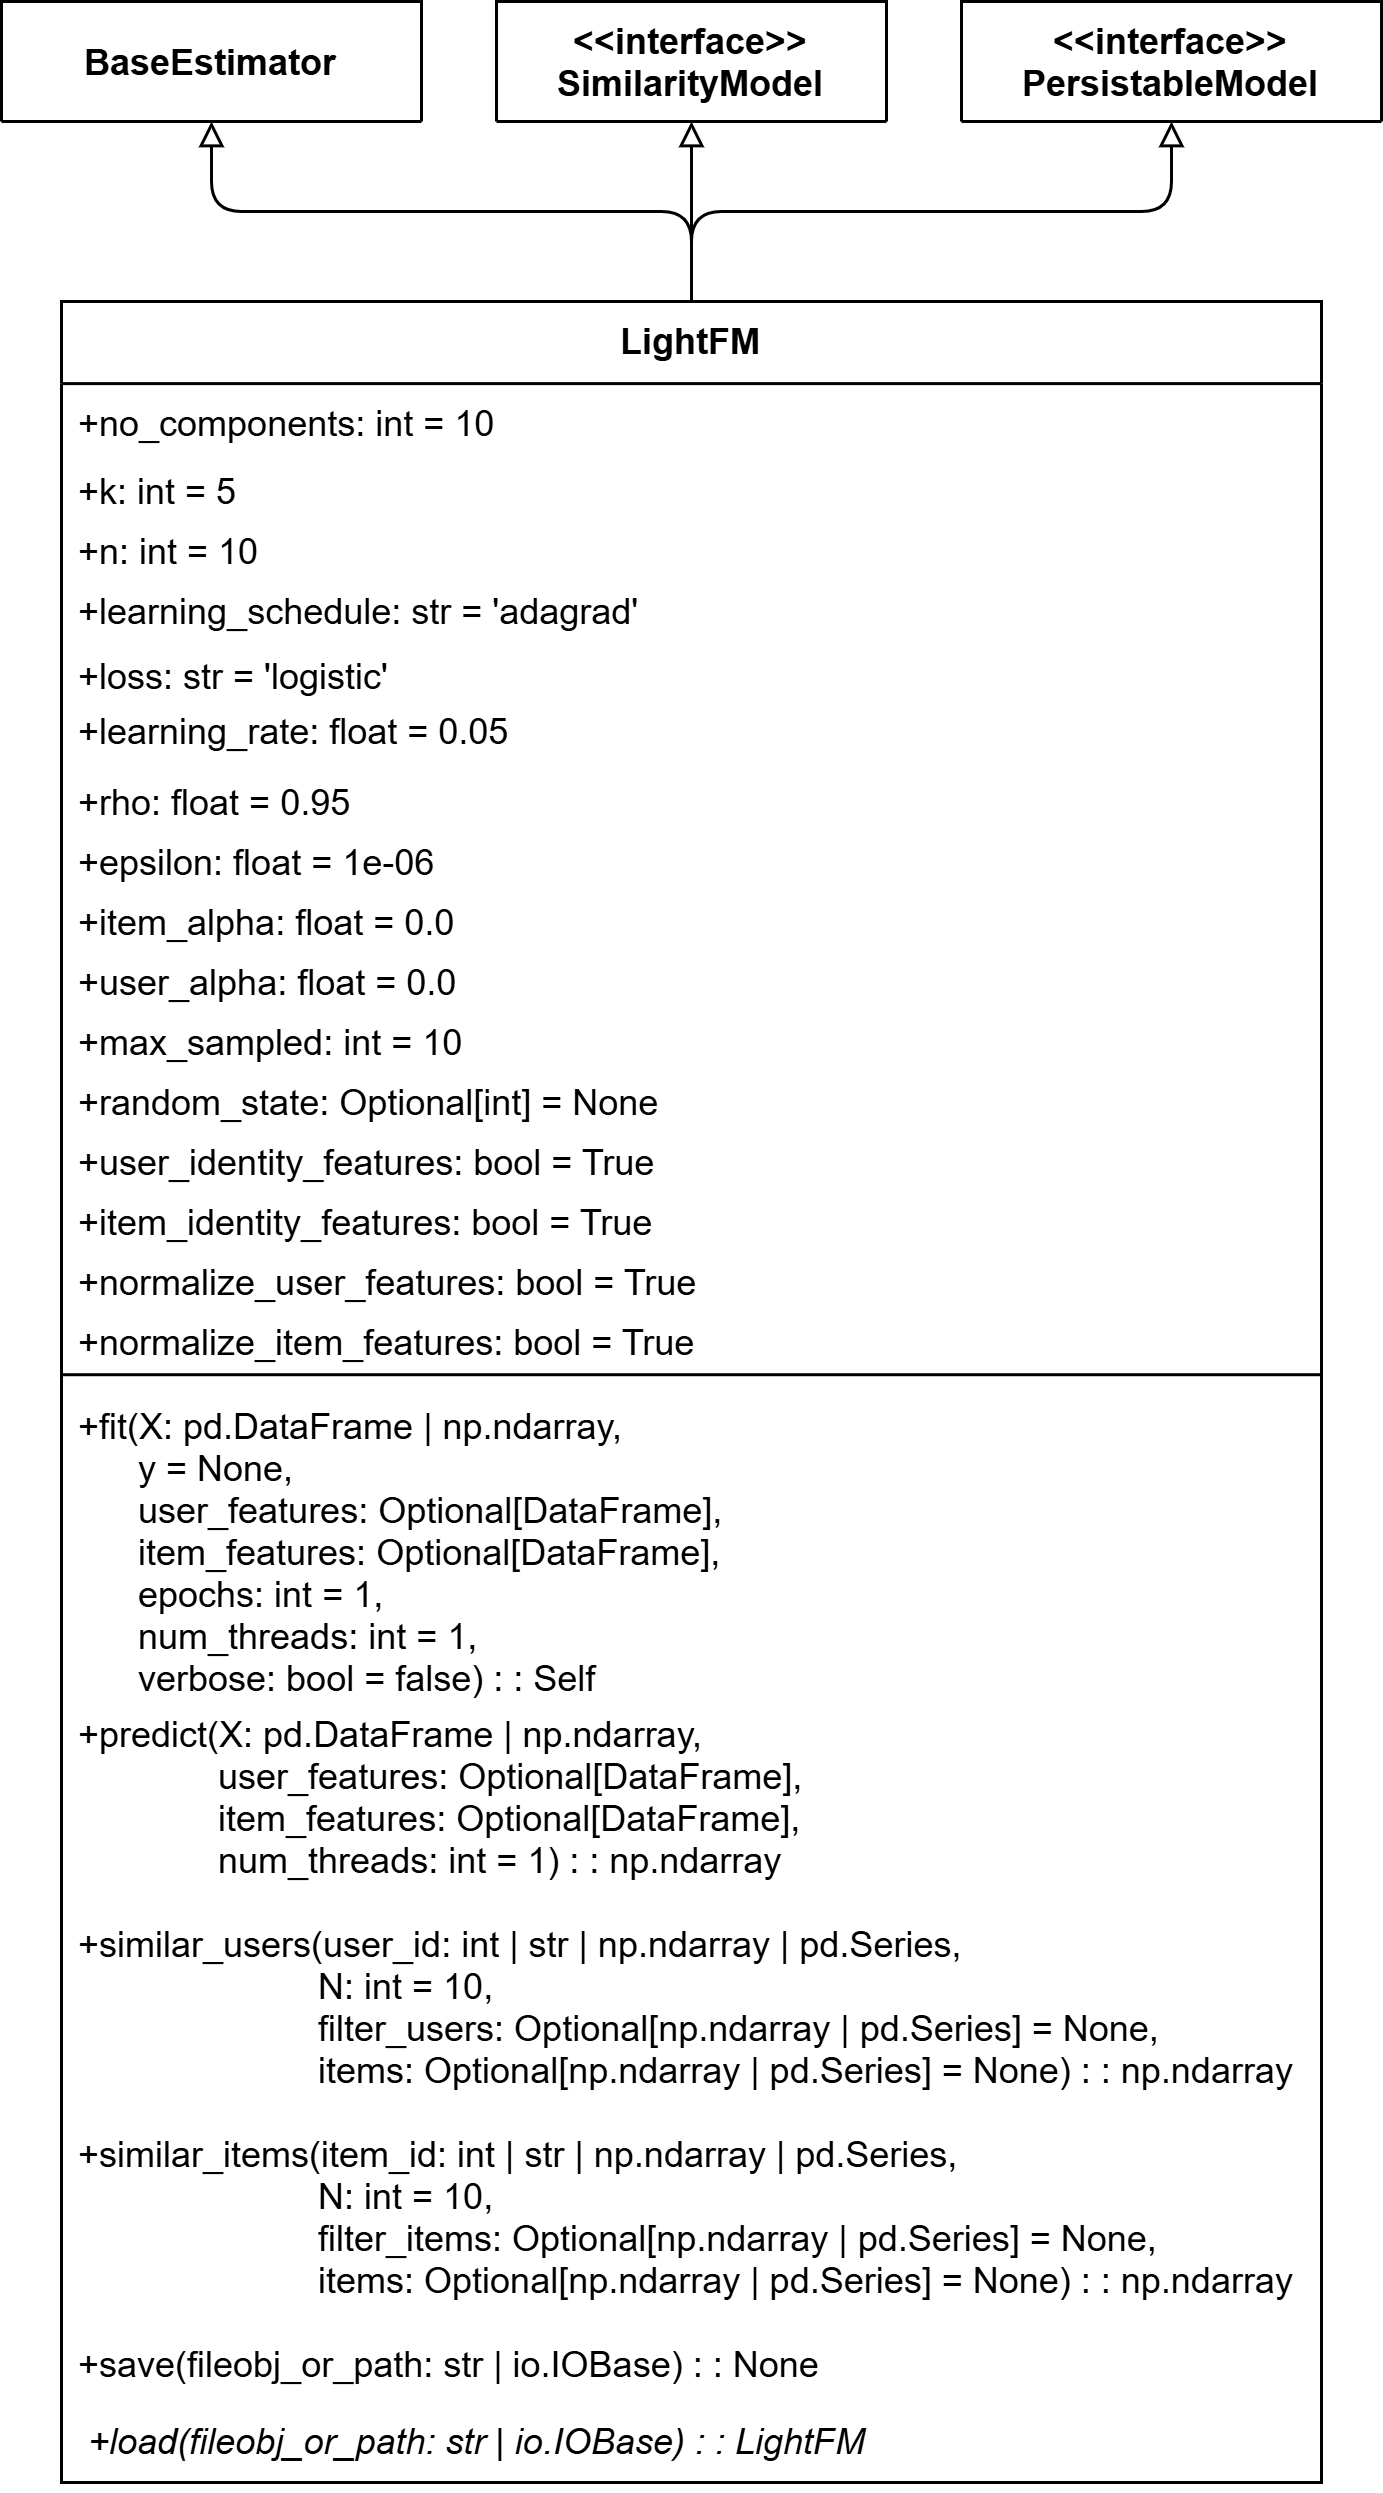
\includegraphics[scale=0.2]{figures/UML/models/light_fm.png}
    \caption{Diagrammi della classe \textit{LightFM}}
\end{figure}

\subsubsection{Costruttore}

Il costruttore riceve gli stessi parametri del modello originale della libreria \textit{LightFM} più quattro parametri extra:

\begin{itemize}
    \item \texttt{user\_identity\_features} (\texttt{bool}): crea una feature unica per ogni \textit{user} in aggiunta alle altre features. Se impostato su \texttt{True} (il valore di default), verrà allocato un vettore latente per ogni \textit{user}.  Questo è un valore predefinito ragionevole per la maggior parte delle applicazioni, ma dovrebbe essere impostato su \texttt{false} se sono disponibili pochissimi dati per ciascun \textit{user}. Per ulteriori dettagli, consultare le \textit{Note} sulla documentazione di \textit{LightFM}
    \item \texttt{item\_identity\_features} (\texttt{bool}): crea una feature unica per ogni \textit{item} in aggiunta alle altre features. Se impostato su \texttt{True} (il valore di default), verrà allocato un vettore latente per ogni \textit{item}. Questo è un valore predefinito ragionevole per la maggior parte delle applicazioni, ma dovrebbe essere impostato su \texttt{false} se sono disponibili pochissimi dati per ciascun \textit{item}. Per ulteriori dettagli, consultare le \textit{Note} sulla documentazione di \textit{LightFM}
    \item \texttt{normalize\_user\_features} (\texttt{bool}): se impostato su \texttt{True} (il valore di default), il modello utilizzerà, per l'addestramento, una versione normalizzata delle feature degli \textit{user}, garantendo che i pesi delle features sommino a 1 in ogni riga
    \item \texttt{normalize\_item\_features} (\texttt{bool}): se impostato su \texttt{True} (il valore di default), il modello utilizzerà, per l'addestramento, una versione normalizzata delle feature degli \textit{item}, garantendo che i pesi delle features sommino a 1 in ogni riga
\end{itemize}

\subsubsection{User e Item features}

\textit{LightFM} può utilizzare, sia per l'addestramento che per la predizione, informazioni aggiuntive, che corrispondono alle features di \textit{user} e di \textit{item}. 

Ciascun \textit{DataFrame} in input deve seguire la seguente struttura:
\begin{itemize}
    \item devono avere nella prima colonna tutti gli id, per \texttt{user\_id} o \texttt{item\_id}, che compaiono nel \textit{trainset}
    \item le colonne successive devono essere avere un titolo
\end{itemize}

Le stesse considerazioni valgono per le features degli \textit{user}.

Non è obbligatorio specificare entrambe le features contemporaneamente.

\begin{table}[H]
    \centering
    \begin{tabular}{|c|c|c|c|c|}
    \hline
    \textbf{item\_id} & \textbf{genre} & \textbf{pages} & \textbf{year} & \textbf{author} \\
    \hline
    B001 & Fantasy       & 432 & 2010 & Luca Ferri       \\
    B002 & Giallo        & 289 & 1998 & Martina Rossi     \\
    B003 & Sci-Fi        & 521 & 2022 & Giovanni Bianchi  \\
    B004 & Storico       & 376 & 1985 & Elena Neri        \\
    B005 & Romanzo       & 645 & 2001 & Paolo Conti       \\
    \hline
    \end{tabular}
    \caption{Esempio di \texttt{item\_features} con features su libri}
    \label{tab:book_metadata}
\end{table}

\subsubsection{Modifiche ai metodi}

Il metodo \texttt{fit} di questo modello può ricevere cinque parametri extra:

\begin{itemize}
    \item \texttt{user\_features} (\texttt{DataFrame}): matrice delle features degli \textit{user}. Il valore di default è \texttt{None}
    \item \texttt{item\_features} (\texttt{DataFrame}): matrice delle features degli \textit{item}. Il valore di default è \texttt{None}
    \item \texttt{epochs} (\texttt{int}): numero di epoche da eseguire. Il valore di default è 1
    \item \texttt{num\_threads} (\texttt{int}): numero di thread da utilizzare. Non dovrebbe essere impostato maggiore del numero di core fisici. Il valore di default è 1
    \item \texttt{verbose} (\texttt{bool}): se stampare messaggi durante l'addestramento. Se \texttt{tqdm} è installato, verrà mostrata una barra con il progresso. Il valore di default è \texttt{False}
\end{itemize}

Il metodo \texttt{predict} di questo modello può ricevere tre parametri extra:

\begin{itemize}
    \item \texttt{user\_features} (\texttt{DataFrame}): matrice delle features degli \textit{user}. Il valore di default è \texttt{None}
    \item \texttt{item\_features} (\texttt{DataFrame}): matrice delle features degli \textit{item}. Il valore di default è \texttt{None}
    \item \texttt{num\_threads} (\texttt{int}): numero di thread da utilizzare. Non dovrebbe essere impostato maggiore del numero di core fisici
\end{itemize}

\section{Model Selection}

Il modulo contiene le funzioni per poter eseguire lo split del 
\textit{dataset} in \textit{trainset} e \textit{testset}. La principale, chiamata \texttt{train\_test\_split\_with\_coverage}, riceve in ingresso un \textit{DataFrame} o un \textit{NumPy array} che deve rispettare il formato standard definito sui dati che utilizzano i modelli~\ref{model_fit_data}. 

Lo \textit{split} viene effettuato in modo che nel \textit{trainset} ci sia almeno un'interazione per ogni \textit{user} e ogni \textit{item} in modo che, durante la \textit{prediction}, sia possibile generare un risultato per qualunque \textit{user}/\textit{item} presente durante la fase di \textit{training}. Non ci sono invece sicurezze sul fatto che nel \textit{testset} ci sia, per ogni \textit{user}/\textit{item}, almeno un'interazione. Questo potrebbe portare ad un caso particolare di \textit{cold-start} nel \textit{testset}.

Nel caso in cui non il modello non avesse problemi a gestire \textit{ids} mai visti durante la fase di addestramento e si vuole lavorare esclusivamente con \textit{DataFrame} è possibile utilizzare la seconda ed ultima funzione del modulo chiamata \texttt{random\_train\_test\_split} che effettua uno \textit{split} casuale del \textit{dataset} in \textit{trainset} e \textit{testset} senza alcun vincolo.


\section{Model Evaluation}
Il modulo comprende l'insieme delle funzioni per calcolare le prestazioni dei modelli addestrati.

Per i modelli che gestiscono feedback espliciti sono presenti i seguenti algoritmi:

\begin{itemize}
    \item Root Mean Squared Error (RMSE) con la funzione \texttt{rmse}
    \item Mean Absolute Error (MAE) con la funzione \texttt{mae}
\end{itemize}

mentre per quelli che gestiscono feedback impliciti:

\begin{itemize}
    \item Precision@K con la funzione \texttt{precision\_at\_k}
    \item Recall@K con la funzione \texttt{recall\_at\_k}
    \item F1@K con la funzione \texttt{f1\_at\_k}
    \item Hit@K con la funzione \texttt{hit\_at\_k}
    \item Area Under the ROC Curve (AUC) con la funzione \texttt{auc}
    \item Normalized Discounted Cumulative Gain (NDCG) con la funzione \texttt{ndcg}
\end{itemize}

Tutte queste funzioni

\section{Utils}

Il modulo \texttt{utils} raccoglie un insieme di funzioni ausiliarie progettate per supportare attività comuni nella fase di preparazione dei dati e predizione nei modelli di raccomandazione. Le funzioni sono pensate per essere modulari, riutilizzabili e indipendenti dalla specifica implementazione del modello.

\begin{itemize}
    \item \texttt{check\_model\_inputs}: funzione di validazione degli input forniti a un modello. Controlla che tutte le colonne richieste siano presenti, che i dati siano nel formato standard (vedere~\ref{model_fit_data} e~\ref{model_predict_data}) e che rispettino le specifiche attese dal modello. Può essere inclusa nei metodi \texttt{fit} e \texttt{predict} dei modelli che accettano i dati nel formato standard

    \item \texttt{generate\_user\_item\_pairs}: prende in input una matrice (in formato \textit{DataFrame} o \textit{NumPy array}) che contiene almeno due colonne: la prima con gli \texttt{user\_id} e la seconda con gli \texttt{item\_id}. Le eventuali colonne aggiuntive vengono ignorate. La funzione genera un \textit{DataFrame} contenente tutte le coppie possibili (\texttt{user\_id}, \texttt{item\_id}) ottenute dal prodotto cartesiano tra gli \textit{user} e gli \textit{item} presenti nei dati forniti. Questo serve affinché i modelli possano calcolare, tramite il metodo \texttt{predict}, il \textit{ranking} di tutti gli \textit{item} per ciascuno \textit{user}
    \begin{table}[H]
        \centering
        \begin{minipage}{\textwidth}
            \centering
            \textbf{Input (user\_id, item\_id)}\\[0.5em]
            \begin{tabular}{|c|c|c|}
            \hline
            \textbf{user\_id} & \textbf{item\_id} & \textbf{timestamp} \\
            \hline
            1 & 10 & 2025-01-01 \\
            2 & 11 & 2025-01-02 \\
            3 & 12 & 2025-01-03 \\
            \hline
            \end{tabular}
        \end{minipage}

        \vspace{1em} % Spazio verticale tra le tabelle

        \begin{minipage}{\textwidth}
            \centering
            \textbf{Output (prodotto cartesiano)}\\[0.5em]
            \begin{tabular}{|c|c|}
            \hline
            \textbf{user\_id} & \textbf{item\_id} \\
            \hline
            1 & 10 \\
            1 & 11 \\
            1 & 12 \\
            2 & 10 \\
            2 & 11 \\
            2 & 12 \\
            3 & 10 \\
            3 & 11 \\
            3 & 12 \\
            \hline
            \end{tabular}
        \end{minipage}
        \caption{Esempio di input e output per \texttt{generate\_user\_item\_pairs}}
    \end{table}
\end{itemize}


\section{Visualization}
Il modulo comprende l'insieme delle funzioni di supporto dedicate all'analisi esplorativa e alla visualizzazione di dati in formato \textit{DataFrame}. In particolare, fornisce strumenti per rappresentare graficamente la distribuzione di variabili continue e categoriali tramite istogrammi, curve di densità e grafici a barre, facilitando la comprensione della frequenza e della percentuale dei valori presenti. Inoltre, include una funzione principale, \texttt{describe}, che, data una struttura dati tabellare, consente di visualizzare in modo personalizzato le distribuzioni di colonne categoriali e continue, supportando anche colonne con valori multipli separati da un delimitatore.

Questo modulo è stato pensato per poter visualizzare ed analizzare le distribuzioni di eventuali \textit{rating} e features di \textit{user} e \textit{item}.

\begin{itemize}

  \item \texttt{plot\_hist}: è una funzione per visualizzare la distribuzione di una variabile continua sotto forma di istogramma. Utilizza la libreria \texttt{seaborn} per generare il grafico, con la possibilità di specificare il numero di intervalli (\texttt{bins}) oppure lasciare che vengano determinati automaticamente. È utile per esplorare la frequenza dei valori e la forma generale della distribuzione (simmetrica, asimmetrica, ecc.)

  \item \texttt{plot\_continuous\_distribution}: genera una stima della densità di probabilità di una variabile continua tramite il metodo \texttt{kdeplot} (Kernel Density Estimation). Questo tipo di grafico è utile per comprendere la forma teorica della distribuzione, in modo più fluido e continuo rispetto all'istogramma, mettendo in evidenza eventuali picchi, code o multi-modalità nei dati.

  \item \texttt{plot\_categorical\_distribution}: visualizza la distribuzione di una variabile categorica. Può opzionalmente suddividere valori multipli contenuti in una singola cella (e.g. stringhe separate da virgole) tramite \textit{split}. I valori vengono contati e mostrati in un grafico a barre orizzontali, con etichette descrittive che indicano il numero assoluto e la percentuale relativa di ciascuna categoria. È particolarmente utile per analizzare la frequenza delle classi o delle etichette presenti nei dati

  \item \texttt{describe}: è una funzione riassuntiva che combina più strumenti di esplorazione visiva per un'intero \textit{DataFrame}. Permette di specificare quali colonne siano categoriche, continue o da visualizzare tramite istogrammi, e genera automaticamente i grafici appropriati per ciascuna tipologia. È pensata per offrire un'esplorazione iniziale rapida dei dati, facilitando l'analisi preliminare tramite visualizzazioni mirate. Può anche stampare il contenuto del \textit{DataFrame} se richiesto

\end{itemize}